\documentclass{article}
\usepackage{fullpage}
\usepackage{parskip}
\usepackage{standalone}
\usepackage{graphicx}
\usepackage{booktabs}
\usepackage{subcaption}
\usepackage{hyperref}
\usepackage{xurl}
\usepackage{amsmath}
\usepackage{amsfonts}
\usepackage{amsthm}
\usepackage{xfrac}
\usepackage{enumitem}
\usepackage[table]{xcolor}
\usepackage{minted}
\usepackage{xfrac}
\usepackage{tikz}
\usetikzlibrary{arrows}
\usetikzlibrary{decorations.pathreplacing}
\usetikzlibrary{calc}
\usetikzlibrary{shapes.geometric}
\usetikzlibrary{decorations.markings}
\usetikzlibrary{shapes.geometric}
\usetikzlibrary{patterns,snakes}
\usetikzlibrary{decorations.text}
\usetikzlibrary{arrows.meta}

\definecolor{codebg}{RGB}{255, 255, 230}
\setminted[python]{
    frame=single,
    framesep=2mm,
    bgcolor=codebg,
    framerule=0.5mm,
    fontsize=\normalfont,
}

\newtheorem{prop}{Proposition}


\title{Queues Under Stochastic Priority Switching}
\author{Geraint I. Palmer, Michalis Panayidis, Vincent Knight \& Elizabeth Williams}
\date{}

\begin{document}
\maketitle

\begin{abstract}
In this paper a generalised model of dynamic and stochastic changing priorities
within an $M/M/c$ queue is presented. Simulation and Markov chain models are
given that describe the behaviour of such systems, and their stationarity is
explored.
Bounded approximations of the Markov models are given, and measures of their
accuracy in approximating the infinite versions given. Finally the models are
used to model a waiting list for surgical endoscopy with unknown service
disciplines, fitting system parameters to reflect the queue behaviour. An
exploration of behaviour under different class change parameters is given for a
better understanding of the system. 
\end{abstract}

\section{Introduction}
There are a number of situations in which a customer's priority in a queue might
change during their time queueing, or equivalently where their priority depends
on the amount of time they have already spent in the queue.
Classic examples arise in healthcare systems, for example when a patient's
medical urgency increases the longer they spend waiting due to health
degeneration \cite{williams20, garbuzetal06, delongetal08}. Another example
would be a prioritisation scheme that attempts a trade-off between medical need
and waiting times \cite{powersetal23}.
These are both examples where a patient's priority has the chance to upgrade
over time while in the queue.
However there also might be situations in which a patient's priority can
downgrade over time: consider a medical intervention that can improve a
patient's outcome if caught early, if a patient has been waiting a long time
already then they might be passed over for a newly referred patient who will
gain more benefit from the intervention. In this case a patient's priority is
downgraded the longer they wait \cite{dalessandro17}.

In this paper a single $M/M/c$ queue is modelled, with multiple classes of
customer of different priorities. While waiting in the queue, customers change
their class to any other class at specific rates. Thus upgrades, downgrades, and
`skip-grades' (moving to a priority class not immediately above or below the
current class) are modelled.

This is first modelled using simulation, where we describe generalisable logic.
This was first implemented in version v2.3.0 of the Ciw library in Python
\cite{palmer19} and is a contribution of this paper.
An important question arises from this, when does a steady state distribution
exist for such a queueing system? To answer this question, two Markov chain
models are defined, which are used to find
steady state distributions and expected sojourn times for each customer class.
These Markov chains give some insights into the behaviour of the systems under
different combinations of parameters; and numerical experiments give further
behaviours.

This paper is structured as follows:
Section~\ref{sec:casestudy} gives a motivating example from a healthcare
setting demonstrating the need for this type of model.
Section~\ref{sec:related} highlights some previous and related work.
Section~\ref{sec:system} defines the system under consideration in detail.
Section~\ref{sec:simulation} discusses the simulation logic required and the
contribution to the Ciw library; then experimentally justifies the use of these
models to model scenarios where prioritisation rules are unknown.
Section~\ref{sec:makovchains} defines two Markov chain models of the system, one
useful for considering system-wide statistics such as state probabilities, and
one useful for considering customers' statistics such as average sojourn time.
This includes exploring a bounded approximation for numerically tractable
analysis, presenting measures of accuracy for these bounded approximations, and
discussing the existence or otherwise of systems that can reach steady state.
An exploration of the system behaviour under different parameters is given.

\subsection{Motivating Case Study}\label{sec:casestudy}
Consider the queueing process for a particular surgical procedure. In many cases
the service discipline, that is the rules for how patients chosen from the
waiting list to be scheduled for surgery, are not known to modellers, and may
even be impossible to know as managers may be reluctant to disclose the
information for political or other reasons.
We consider and investigate the waiting list of a surgical
endoscopy procedure carried out in the Cardiff and Value University Health Board
(CAVUHB) over the period 1st January to 31st December 2021.

It is clear from examining the data that a first-in-first-out (FIFO) service
discipline was not used. To show this, we assign each patient in the data set
an arrival rank, the order in which they were referred for an endoscopy, and a
service rank, the order in which they received their endoscopy. The difference
in the two ranks corresponds to the net number of patients that they `overtook'
in the queue: a negative number indicates more customers overtook them, we'll
say they were `bumped down' the queue; while a positive number indicates that
they overtook more people, and we'll say they were `bumped up' the queue. During
the observation period, 169 patients received an endoscopy, and
Figure~\ref{fig:motivating_overtakes} shows the distribution of the rank
differences, and the distribution of waiting times by those who were bumped up
or down the queue. No patient had a waiting time of zero, indicating that no
patient was referred to the queue in a prioritised state, hinting that patients
may have priorities that change over time.
The figure also reports $\omega_{\uparrow}$ and $\omega_{\downarrow}$, the
average waiting time for patients that were bumped up and down the list,
respectively.

\begin{figure}
  \begin{center}
    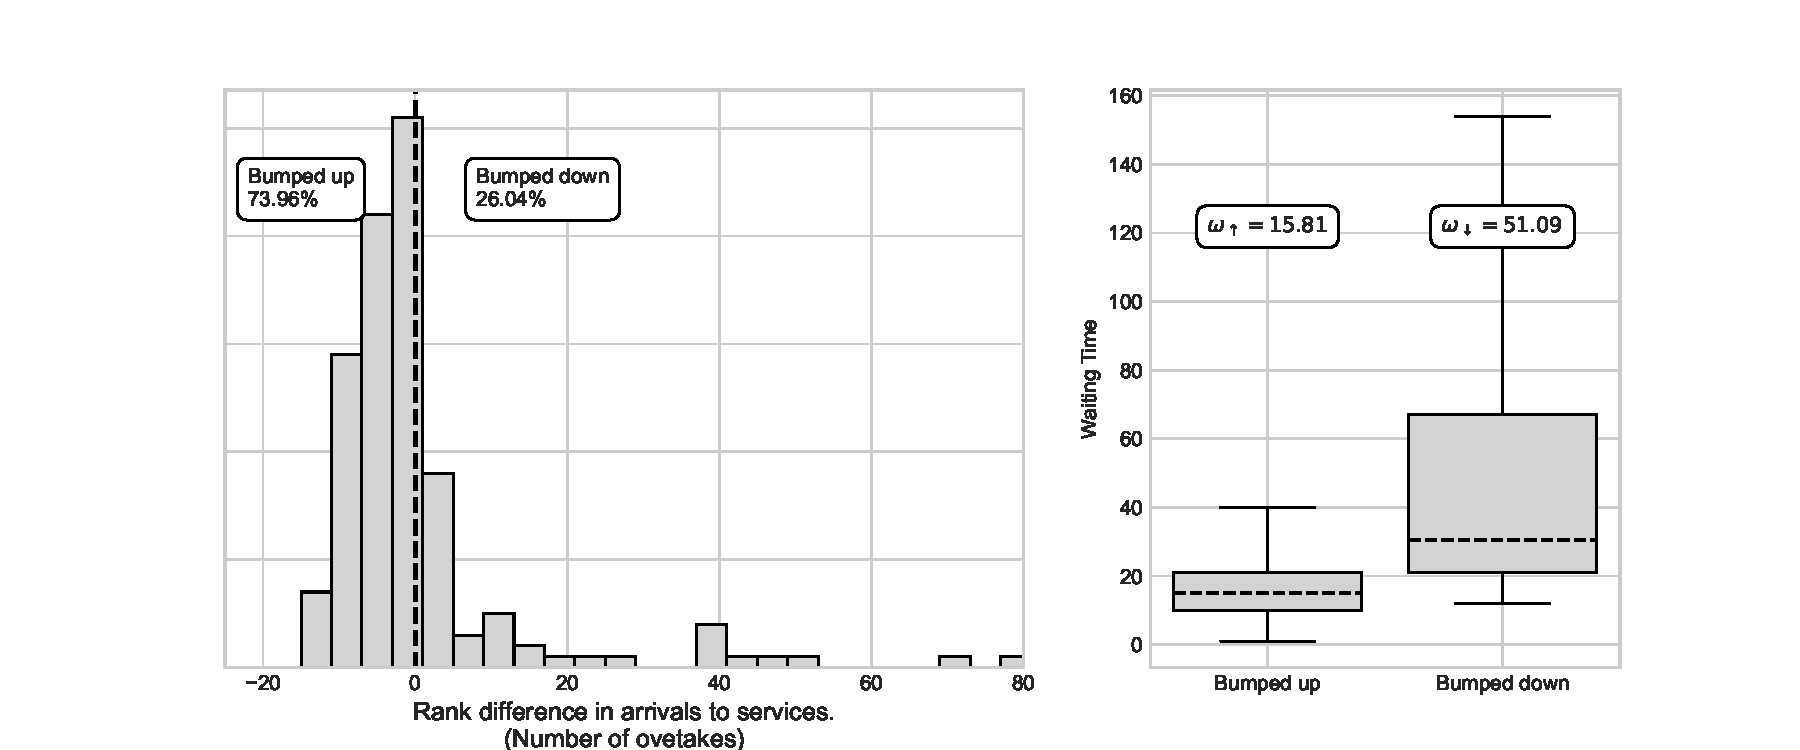
\includegraphics[width=\textwidth]{img/motivating_overtakes.pdf}
  \end{center}
  \caption{Distribution of overtakes in a CAVUHB endoscopy waiting list.}
  \label{fig:motivating_overtakes}
\end{figure}

\subsection{Related Work}\label{sec:related}
Systems of this kind have been investigated previously:

\begin{itemize}
  \item \cite{jackson60} (1960): Non pre-emptive $M/M/1$ where customers
      are served in order of the difference between their waiting time
        and urgency number (that is priorities increasing linearly over
        time). Solved by considering event probabilities at clock ticks.
  \item \cite{kleinrock164} (1964): Another formulation giving the same
      behaviour as \cite{jackson60}, but now for both non pre-emptive and
        pre-emptive priorities, and multiple customer classes. Called `delay
        dependent' or `time dependant' priorities, and recently by
        `accumulating' priorities.
  \item \cite{adiri71} (1971): Introduces a model where customers are
      de-prioritised during service if their service time exceeds a given
        minimum time interval, or quantum of time. Customers are downgraded and
        made to wait again for service, behind newly arriving and newly
        downgraded customers.
  \item \cite{holtzman71} (1971): Similar to \cite{jackson60}, but treat each
      urgency number as a separate customer class, and not considering
        clock ticks. Upper and lower bounds on the waiting times, based
        on FIFO and static priorities.
  \item \cite{netterman79} (1979): Now considers the case where
      priorities increase non-linearly but concavely over time.
  \item \cite{bagchisullivan85} extends the work of
      \cite{jackson60, kleinrock164, holtzman71} by considering cases where the
        multiple classes of customer have less restrictive orderings of the
        linear priority functions.
  \item \cite{fratini90} (1990): Non pre-emptive $M/G/1$ queue with two
      classes of customers, where priorities switch if the number from
        one class exceeds a given threshold. Lower priority customers
        have a finite waiting capacity, higher have infinite capacity.
  \item \cite{vanmieghan95} (1995): Introduces the generalised $c\mu$-rule
    (first conceived in \cite{smith56}), which applies a class- and waiting
      time-dependant cost to each customer. This acts as a scheduling rule,
      but can also model changing priorities amongst customers.
  \item \cite{xhafa01} (2001): Models calls in personal communication systems.
      It considers system with three priority classes, the lower priority class
      is lost to the system when servers are busy, while the other two classes
      experience non-pre-emptive priorities, and exponentially distributed
      upgrades from the middle priority to the highest priority.
  \item \cite{knessl03} (2003): Similar to \cite{fratini90} but with Markovian
      services and infinite waiting capacities for both customers.
  \item \cite{xie08} (2008): Pre-emptive n-priority-classes $M/M/c$ with
      exponential upgrades. Customers only upgrade to the priority
        immediately higher than themselves. Stability considered.
  \item \cite{down10} (2010): Pre-emptive two-priority-classes $M/M/c$ with
      exponential upgrades. Customers cannot upgrade if the number of
        lower priority customers is below a given threshold. Holding
        costs considered.
  \item \cite{he12} (2012): Extension of \cite{down10}, allows batch
      arrivals, multiple classes, phase-type upgrades and services.
        Customers only upgrade to the priority immediately higher than
        themselves.
  \item \cite{stanford14} (2014): Furthers the work of \cite{kleinrock164} to
      look at the maximum priority of the waiting customers in a single server
        queue as a stochastic process termed an accumulating priority queue
        (APQ). This is extended in \cite{sharif14} to multi-server queues, in
        \cite{li2016} to account for heterogeneous servers, and in \cite{li2017}
        to find non-linear accumulation functions that are equivalent to linear
        ones.
  \item \cite{kella17} (2017): Derives waiting time distributions for queues
      with multiple classes of customer and class-dependent priority
        accumulation rates, where priorities accumulate linearly over time.
  \item \cite{ferrandetal18} (2018): Shows that by using the \cite{kleinrock164}
      setup in a simulation of a ED in a children's hospital leads to more
        efficient resource use.
  \item \cite{klimenok20} (2020): Upgrades and downgrades after a random,
      exponentially distributed, amount of time. Models two priority classes
        in a single server, finite buffer system with batch arrivals. Extended
        in \cite{leeetal20} to include multiple priority classes but without
        downgrades, and in \cite{dudin21} to include unreliable services and
        impatient customers. 
  \item \cite{bilodeau22} (2022): Analytical (truncated) expressions for
      a two class delayed accumulating priority $M/G/1$ queue. Customer
        priorities increase linearly over time, at different rates
        according to class, after an initial fixed delay.
\end{itemize}


\begin{itemize}
  \item \cite{ding19} (2019): Evidence that in Canada that decision makers
      often use their own discretion in deciding which patients to be seen,
        rather than FIFO within each triage category. Fits prioritisation rules
        to this discretionary behaviour.
\end{itemize}




\section{An $M/M/c$ queue with stochastic priority switching}\label{sec:system}
In this section, we present the detailed description of our queueing model where
customers can stochastically which priority classes while waiting.
Consider an $M/M/c$ queue with $K$ classes of customer labelled
$0, 1, 2, \dots, K-1$. Let:

\begin{itemize}
  \item $\lambda_k$ be the arrival rate of customers of class $k$,
  \item $\mu_k$ be the service rate of customers of class $k$,
  \item $\theta_{i,j}$ be the rate at which customers of class $i$ change
  to customers of class $j$ while they are waiting in line.
\end{itemize}

Customers of class $i$ have priority over customers of class $j$ if $i < j$.
Customers of the same class are served in the order they arrived to that class.
Figure~\ref{fig:twoclass_example} shows an example with two classes of customer.

\begin{figure}
\begin{center}
\includestandalone[width=0.7\textwidth]{img/priority_queue}
\end{center}
\caption{An example of a two-class priority queue.}
\label{fig:twoclass_example}
\end{figure}

The key feature here is the $K \times K$ class change matrix
$\Theta = (\theta_{i,j})$. All elements $\theta_{i,j}$ where $i \neq j$ are
rates, and so are non-negative real numbers, if customers of class $i$ cannot
change to customers of class $j$ directly, then $\theta_{i,j} = 0$. The diagonal
values $\theta_{i,i}$ are unused as customers cannot change to their own class.
All elements $\theta_{i,i-1}$ represent the direct upgrade rates; all elements
$\theta_{i,i+1}$ represent the direct downgrade rates, while all other elements
can be thought of as `skip-grades'.
This is shown in Figure~\ref{fig:skipgrades}.

\begin{figure}
\begin{center}
\includestandalone[width=0.65\textwidth]{img/skipgrades}
\end{center}
\caption{Representations of parts of the matrix $\Theta$. Example when $K=5$.}
\label{fig:skipgrades}
\end{figure}

The priorities are pre-emptive, that is if a newly arriving customer has a
higher priority than a customer in service, or if a waiting customer changes
priority class to a higher priority than a customer is service, then that new
customer displaces the lowest priority customer that is in service. The
displaced customer rejoins the queue, before all other customers of their own or
lower priority classes, but behind all other customers of higher priority
classes. When that displaced customer eventually enters service again, their
service time can either be resumed, re-started, or re-sampled.

The next two sections outline and compare a discrete event simulation and
Markov chain formulations for modelling this setup.



\section{Simulation Model Logic}\label{sec:simulation}
Discrete event simulation is a common way of modelling queueing systems,
especially those with non-standard customer behaviours as the development time
for capturing new or complex behaviours is a lot quicker than Markov modelling
\cite{standfield14}.
One standard way of implementing discrete event simulation is through the event
scheduling approach \cite{robinson14}. This is a variant of the three-phase
approach, with an \textbf{A}-phase which advances the clock to the next
scheduled event, a \textbf{B}-phase where scheduled events are carried out, and
a \textbf{C}-phase where conditional events are carried out.
Figure~\ref{fig:eventscheduling} shows a flow diagram of the logic of the event
scheduling approach.

\begin{figure}
    \centering
    \includestandalone[width=\textwidth]{img/eventschedulingapproach}
    \caption{Flow diagram of the event scheduling approach, adapted from
    \cite{palmer18}.}
    \label{fig:eventscheduling}
\end{figure}

The primary scheduled, or \textbf{B}-events that occur in queueing simulations
are customers arriving to a queue, and customers finishing service.
The conditional, or \textbf{C}-events are those that happen immediately after,
and because of, these \textbf{B}-events. The primary ones are customers
beginning service, and customers leaving the queue.

Any other customer, server, or system behaviour to be captured by the simulation
corresponds to increasing the range of \textbf{B}- and \textbf{C}-events that
can happen during the simulation run. For example if servers are subject to a
work schedule, then extra \textbf{B}-events include a server going off and on
duty, and extra \textbf{C}-events would include include a customer beginning
service after another customer has left the server.

In the case of customers randomly changing priority classes while waiting, one
additional \textbf{B}-event and two additional \textbf{C}-event need to be
included:

\begin{itemize}
  \item Upon arrival to the queue customers are assigned a date in which they
  will change customer class, determined by randomly sampling from a
  distribution. As such each customer's event of changing customer class is
  scheduled for the future, and are therefore \textbf{B}-events. If those
  customers begin service (which might not be scheduled yet) before that event
  has occurred, then their changing customer class event is cancelled.
  \item Upon changing class, they immediately schedule another changing class
  event for the future, again sampling a date from a given distribution. This
  happens immediately after the above, and so is a \textbf{C}-event.
  \item If a newly arriving customer is of a higher priority than a customer in
  service, or if a lower priority customer is upgraded to a higher priority a
  customer in service, then the lower priority customer in service is
  pre-empted. They stop service and are placed at the head of the queue. This
  happens immediately after and arrival or after an upgrade, and so is a
  \textbf{C}-event.
\end{itemize}


\subsection{Ciw Implementation}
In this work we use and adapt the Ciw library \cite{palmer19} to simulation
customers changing priority class. Ciw is an open-source Python library for
discrete-event simulation of open queueing networks. A key contribution of this
work is the adaptation of the library's logic to facilitate the type of
stochastic priority switching described in Section~\ref{sec:system}.
This adaptation was first released in version Ciw v2.3.0, with usage
documentation at
\url{https://ciw.readthedocs.io/en/latest/Guides/CustomerClasses/change-class-while-queueing.html}, and works by considering different classes
of customer and mapping each class to a priority ranking.
Figure~\ref{fig:ciwcode} shows the Ciw code
required to simulate the system with two classes of customer, $\lambda_1 = 1$,
$\lambda_2 = 3$, $\mu_1 = 3$, $\mu_2 = 2$, $c = 1$, $\theta_{12} =1.5$, and
$\theta_{21} = 0.5$, for 365 time units. Here the key parameters are
\mintinline{python}{priority_classes}, which takes a tuple containing a Python
dictionary that maps
customer class labels to priority rankings, and a list of pre-emption options
for each node; and \mintinline{python}{class_change_time_distributions},
defining the time distributions used to describe the time it takes to transfer
from one customer class to another. Note here that the simulation framework is
general enough to define any probability distribution here, and is not
restricted to Exponential distributions.

\begin{figure}
\begin{minted}{python}
>>> import ciw
>>> N = ciw.create_network(
...     arrival_distributions={
...         'C0': [ciw.dists.Exponential(rate=1)],
...         'C1': [ciw.dists.Exponential(rate=3)]
...     },
...     service_distributions={
...         'C0': [ciw.dists.Exponential(rate=3)],
...         'C1': [ciw.dists.Exponential(rate=2)],
...     },
...     number_of_servers=[1],
...     priority_classes=({'C0': 0, 'C1': 1}, ["resample"]),
...     class_change_time_distributions={
...         'C0': {'C1': ciw.dists.Exponential(rate=1.5)},
...         'C1': {'C0': ciw.dists.Exponential(rate=0.5)}
...     }
... )
>>> Q = ciw.Simulation(network=N)
>>> Q.simulate_until_max_time(max_simulation_time=365)
\end{minted}
\caption{Example Ciw code to simulate an $M/M/1$ queue with stochastic priority
switching.}
\label{fig:ciwcode}
\end{figure}

Note that the particular distributions used to sample class change dates in
these cases are generic, and any of Ciw's currently pre-programmed distributions
can be chosen, or custom distributions can also be used. For the systems
described in this paper, we choose Exponential distributions with rates
determined by the class change matrix $\Theta$. Ciw allows options letting
pre-empted customers resume, re-start, or re-sample their service time.

\subsection{Modelling Unknown Service Disciplines}\label{sec:modelling}
The stochastic priority switching model presented in Section~\ref{sec:system}
may be used to model situations where FIFO is not appropriate, but specific
service disciplines may not be known. Recall now the motivating example
discussed in Section~\ref{sec:casestudy}, where it was established that FIFO was
not appropriate but service discipline unknown. Here we attempt to use
stochastic priority switching to model the surgical endoscopy waiting list.

According to the observed data referrals roughly follow a Poisson distribution
with rate 0.463 a day. Service rate data is estimated to be around 0.5
endoscopy procedures a day. To determine the appropriateness of the stochastic
priority switching model here, we model the system as a two class system, with
$\lambda_1 = 0.463$ and $\lambda_2 = 0$, and $\mu_1 = \mu_2 = 0.5$ and $c = 1$,
that is all referrals are of the most urgent, with customers able to be
downgraded and then upgraded during their waiting time. We simulate this
system under different parameters of $\theta_{12}$ and $\theta_{21}$. For each
parameter set we observe one year of referrals, over 5 trials. One KPI of
interest is the amalgamated distribution of rank differences, or overtakes,
over the trials; and we compare that with the
distribution of the original system with indeterminate service discipline. The
Wasserstein distance \cite{mostafaei11} between the modelled and actual
distributions is calculated to measure the models' accuracies in approximating
the indeterminate service discipline.
Another KPI is the mean absolute percentage error, MAPE, between the simulated
and actual average waiting times for patients that with bumped up or down the
waiting list.
Figure~\ref{fig:fitting_theta} compares the modelled and actual distributions of
net rank difference, along with the Wasserstein metric $W$ and MAPE in waiting
times, for all pairs
$\left(\theta_{12}, \theta_{21}\right) \in \{1, 2, 3\}\times\{0, 1, 2\}$. From
this it can be seen that a combination of downgrades and upgrades is required to
fit a good distribution of overtakes, and of the parameters tested
$\theta_{12}=3$, $\theta_{21}=1$ produces the best fit both in terms of
Wasserstein distance and MAPE. This indicates that, with further parameter
tuning, these stochastic priority switching models can be used to model unknown
service disciplines.

\begin{figure}
  \begin{center}
    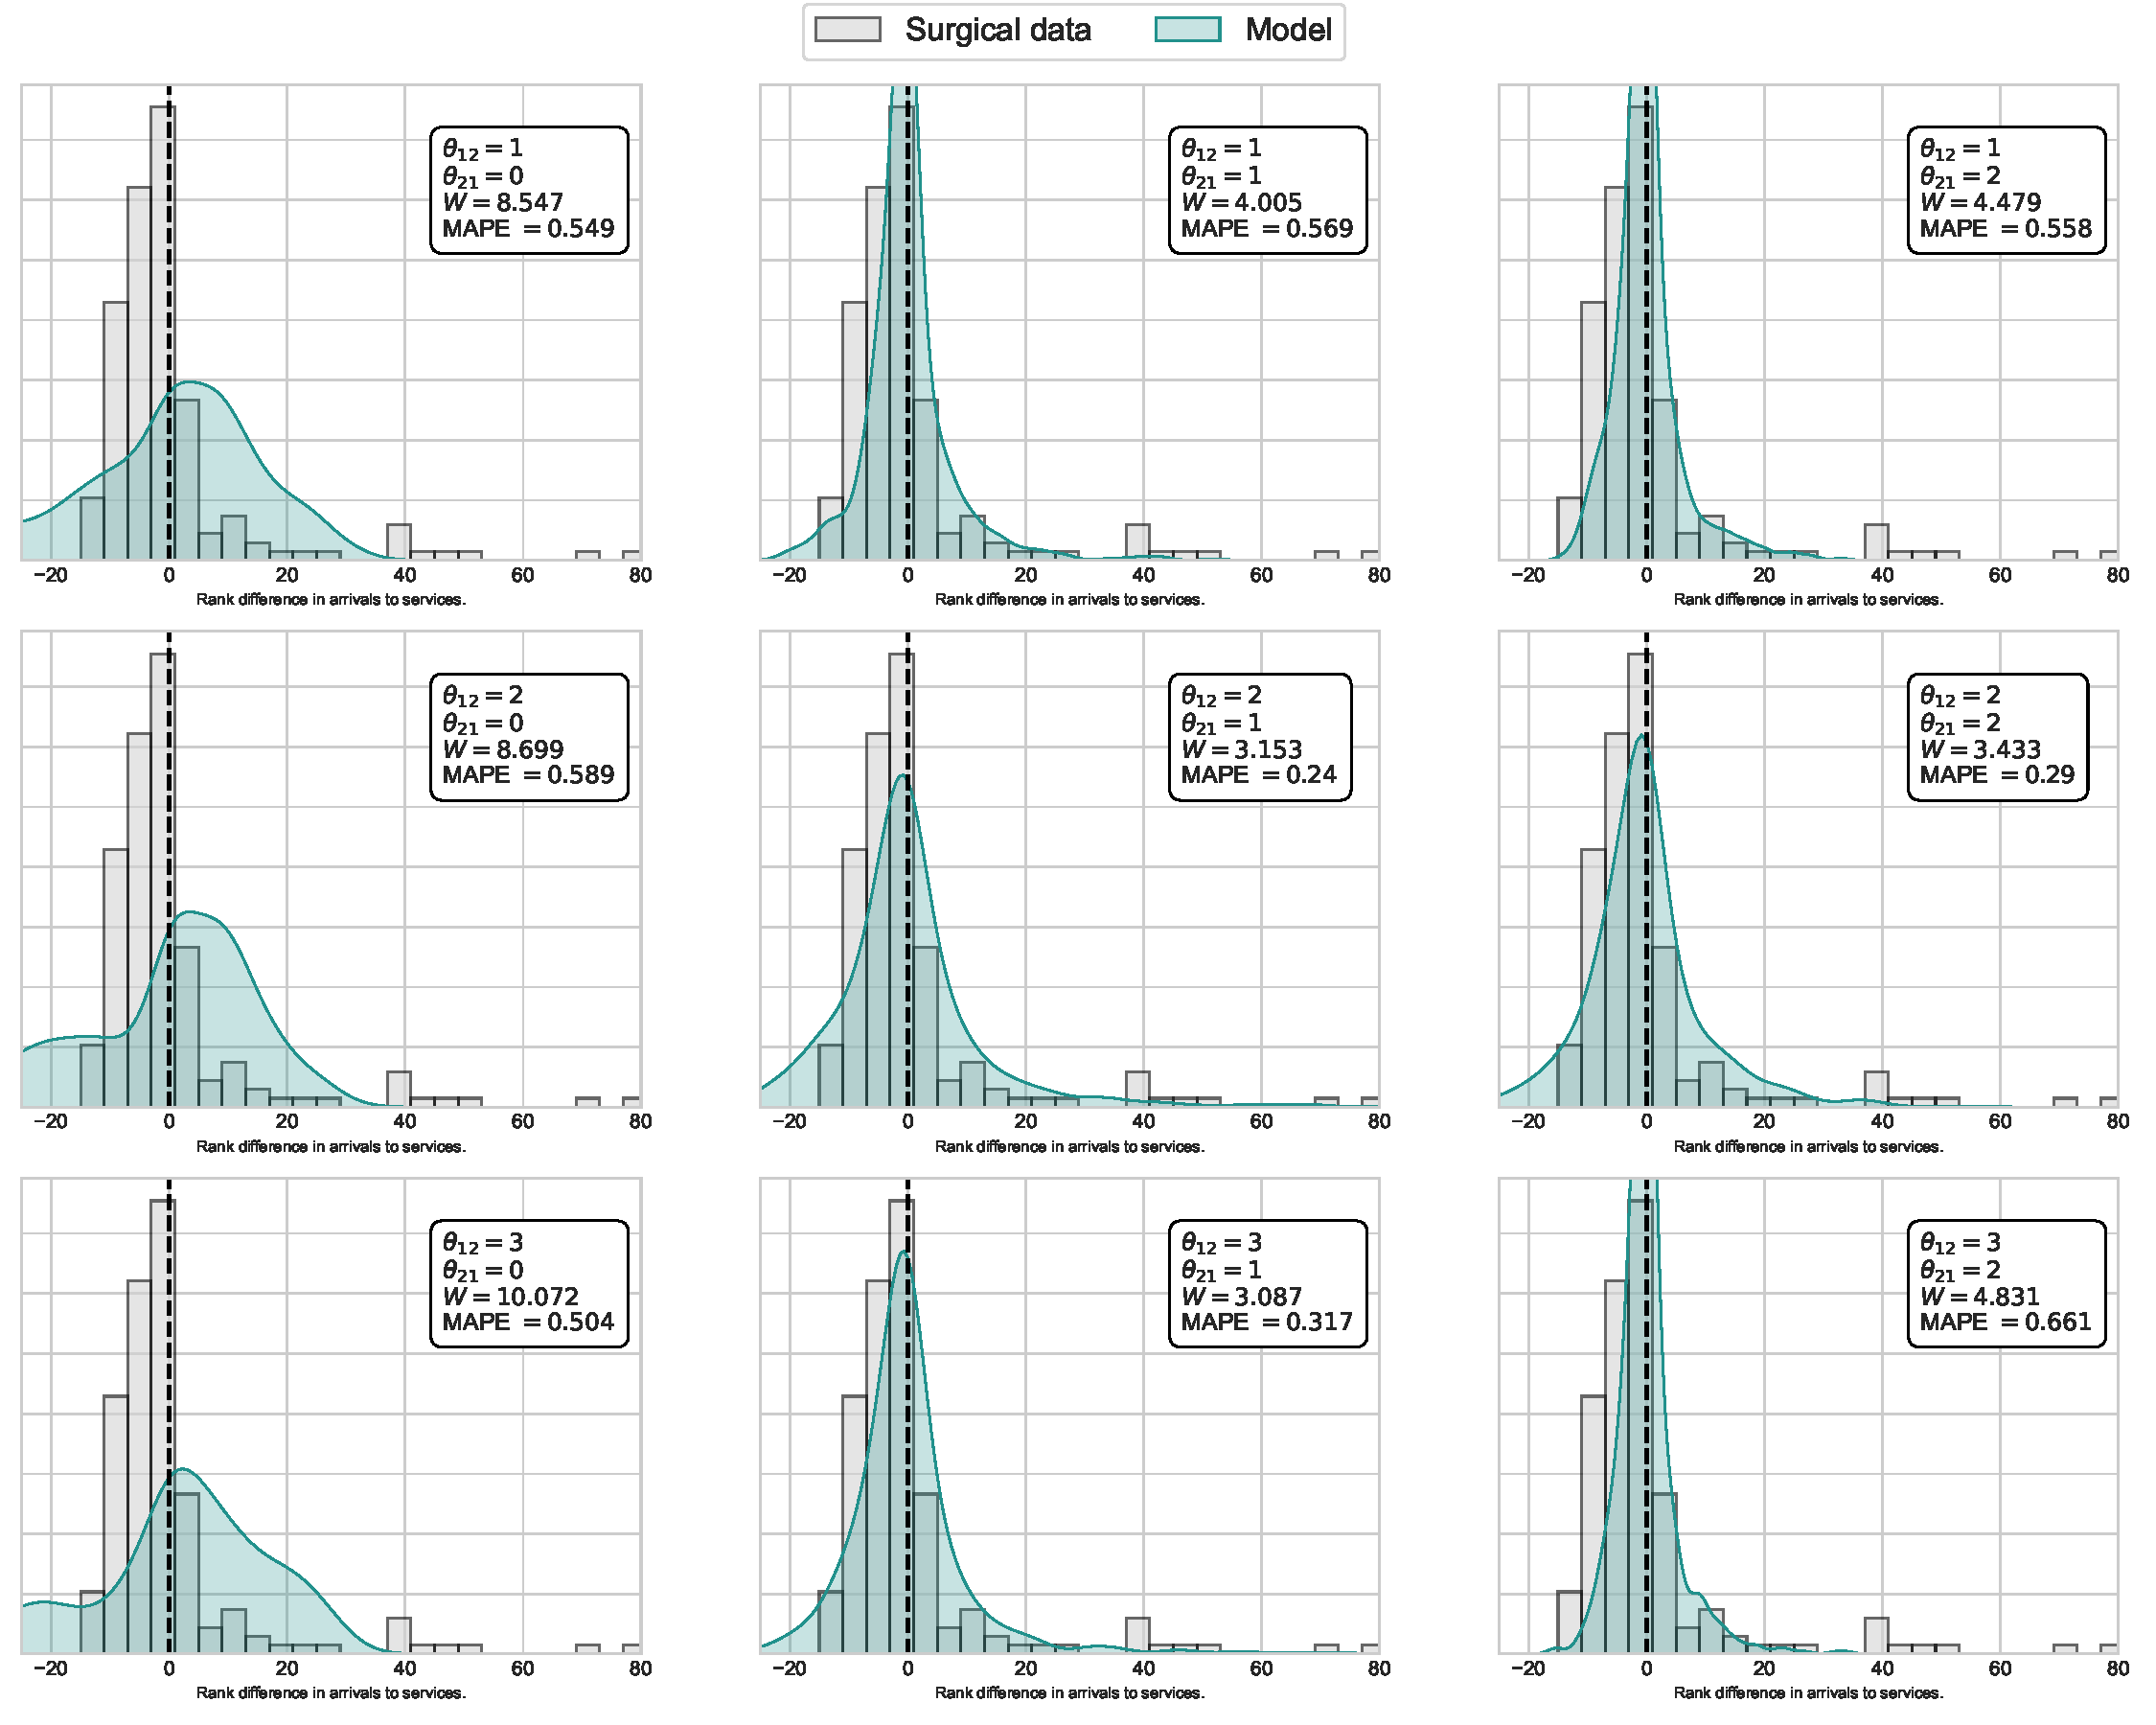
\includegraphics[width=\textwidth]{img/fitting_theta.pdf}
  \end{center}
  \caption{Comparison between simulated and observed overtakes for different
  values of $\theta_{12}$ and $\theta_{21}$.}
  \label{fig:fitting_theta}
\end{figure}

We may then be tempted to use these found values of $\Theta$ to parametrise a
model, to perform standard exercises such as what if scenarios. However we need
more understanding on the dynamics of stochastic priority switching, and in
particular the effect of $\Theta$ and other parameters on the system. As an 
example, consider the case above with $\lambda_1 = 0.463$, $\lambda_2 = 0$,
$c = 1$, and now with $\theta_{12}=3$, $\theta_{21}=1$ as found above. Consider
a small what-if scenario where upgraded customers are served quicker than
downgraded customers, $\mu_1 = 0.4$ and $\mu_2 = 0.6$. Comparing the base
scenario with this new scenario produced vastly different results, in
particular, this new scenario results in an infinitely growing queue, as shown
in Figure~\ref{fig:toy_scenario}.

\begin{figure}
  \begin{center}
    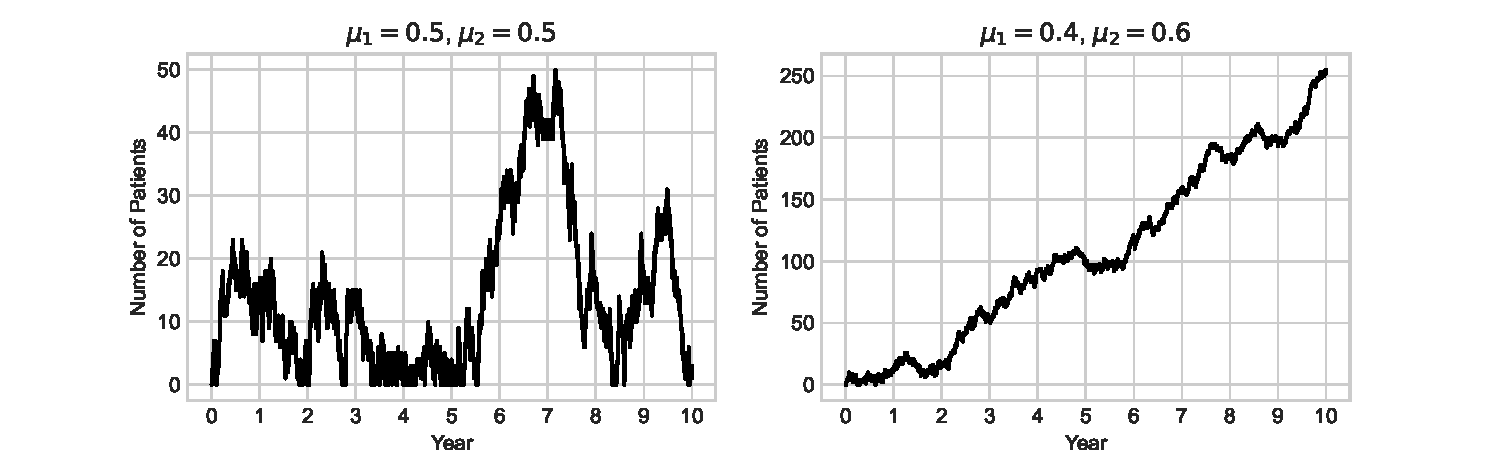
\includegraphics[width=\textwidth]{img/adjust_service_rate.pdf}
  \end{center}
  \caption{Comparison between two simulated scenarios, with stochastic priority
  switching, and differing service rates for each priority. In one scenario the
  queue size reaches a steady state, while in the other the queue size grows
  infinitely.}
  \label{fig:toy_scenario}
\end{figure}

Simulation alone does might not give us sufficient insight into why this occurs.
In the next section we built analytical models of stochastic priority switching,
allowing a deeper insight into the system behaviour.


\section{Markov Chain Models}\label{sec:makovchains}
The situation described in in Section~\ref{sec:system} can be modelled as two
different Markov chains.
The first, described in Section~\ref{sec:state_formulation}, describes the
overall changes in state, where a state records the number of customers of each
priority class present. This is useful for analysing system-wide statistics such
as average queue size.
The second, described in Section~\ref{sec:sojourn_formulation}, describes how an
individual arriving customer experiences the system until their exit. This is
useful for analysing individual customers' statistics such as average sojourn
time.
Given that service times are exponentially distributed and hence memoryless, the
Markov chains are equivalent regardless of whether pre-empted customers resume,
re-start, or re-sample their service.

\subsection{Discrete State Markov Chain Formulation}\label{sec:state_formulation}
Let
$\underline{\mathbf{s}}_t = (s_{0,t}, s_{1,t}, \dots, s_{K-1,t}) \in \mathbb{N}^K$
represent the state of the system at time step $t$, where $s_{k,t}$ represents
the number of customers of class $k$ present at time step $t$. Let $S$ denote
set of all states $\underline{\mathbf{s}}_t$. 

The rates of change between $\underline{\mathbf{s}}_t$ and
$\underline{\mathbf{s}}_{t+1}$ are given by Equation~\ref{eqn:transitions},
where $\underline{\mathbf{\delta}} = \underline{\mathbf{s}}_{t+1} - \underline{\mathbf{s}}_t$,

\begin{equation}\label{eqn:transitions}
q_{\underline{\mathbf{s}}_t, \underline{\mathbf{s}}_{t+1}} = 
\begin{cases}
\lambda_k & \text{if } \delta_k = 1 \text{ and } \delta_i = 0 \; \forall \; i \neq k, \\
B_{k,t} \mu_k & \text{if } \delta_k = 1 \text{ and } \delta_i = 0 \; \forall \; i \neq k \text{ and } \sum_{i < k} s_{i,t} < c, \\
(s_{k,t} - B_{k,t}) \theta_{k,\ell} & \text{if } \delta_{k} = -1 \text{ and } \delta_{\ell} = 1 \text{ and } \delta_i = 0 \; \forall \; i \neq k, \ell, \\
0 & \text{otherwise,}
\end{cases}
\end{equation}

and $B_{k,t}$, representing the number of customers of class $k$ currently in
service at time step $t$, is given by Equation~\ref{eqn:inservice}, where $c$
is the number of servers.

\begin{equation}\label{eqn:inservice}
B_{k,t} =\min\left(c - \min\left(c, \sum_{i < k} s_{i,t}\right), s_{k,t}\right)
\end{equation}

Let $\pi_{\underline{\mathbf{s}}}$ denote the steady state probability of being
in state $\underline{\mathbf{s}} \in S$ (omitting the time step index notation
$t$), while $L_k$ represents the expected number of customers of class $k$, and
$\bar{L}$ represents the total expected number of customers present, given by
Equations~\ref{eqn:mean_custs_k} and~\ref{eqn:mean_custs_overall} respectively.

\begin{equation}\label{eqn:mean_custs_k}
L_k = \sum_{\underline{\mathbf{s}}} \pi_{\underline{\mathbf{s}}} s_k
\end{equation}

\begin{equation}\label{eqn:mean_custs_overall}
\bar{L} = \sum_{k = 0}^{K - 1} \sum_{\underline{\mathbf{s}}} \pi_{\underline{\mathbf{s}}} s_k
\end{equation}



\subsection{Sojourn Time Markov Chain Formulation}\label{sec:sojourn_formulation}
To analyse individual customer statistics, the sojourn time Markov chain
formulation is employed. Let
$\underline{\mathbf{z}}_t = (z_{0,t}, z_{1,t}, \dots, z_{n,t} \dots, z_{K-1,t}, m_t, n_t) \in \mathbb{N}^{K+2} \times (1, \dots, K - 1)$
represent the state of a particular customer at time step $t$, where $n_t$
represents that customer's class at time $t$; $z_{k,t} \; \forall \; k < n$
represents the number of customers of class $k$ in front of the customer in the
queue at time $t$; $z_{k,t} \; \forall \; n < k < K$ represents the number of
customers of class $k$ behind the customer in the queue at time $t$; and $m_t$
represents the number of customers of class $n_t$ behind the customer in the
queue at time $t$.
Also let $\star$ represent an absorbing state, representing the state where that
customer has finished service and left the system.
Let $Z$ denote set of all states $\underline{\mathbf{z}}_t$ and $\star$. 


Then the rates of change between $\underline{\mathbf{z}}_t$ and
$\underline{\mathbf{z}}_{t+1}$ are given by Equation~\ref{eqn:transitions_sojourn},
where $\underline{\mathbf{\delta}} = \underline{\mathbf{z}}_{t+1} - \underline{\mathbf{z}}_t$,

\begin{equation}\label{eqn:transitions_sojourn}
\resizebox{\textwidth}{!}{%
$q_{\underline{\mathbf{z}}_t, \underline{\mathbf{z}}_{t+1}} = 
\begin{cases}
\mu_n & \text{if } z_{t+1} = \star \text{ and } \sum_{k \leq n} z_{k, t} < c, \\
\lambda_n & \text{if } \delta_K = 1 \text{ and } \delta_i = 0 \; \forall \; i \neq K, \\
\lambda_k & \text{if } \delta_k = 1 \text{ and } \delta_i = 0 \; \forall \; i \neq k \text{ and } k \neq n,\\
A_{k,n,t} \mu_k & \text{if } \delta_k = -1 \text{ and } \delta_i = 0 \; \forall \; i \neq k \text{ and } k < K,\\
\tilde{A}_{n,t} \mu_n & \text{if } \delta_K = -1 \text{ and } \delta_i = 0 \; \forall \; i \neq K,\\
(z_{k,t} - A_{k,n,t}) \theta_{k,\ell} & \text{if } \delta_{k} = -1 \text{ and } \delta_{\ell} = 1 \text{ and } \delta_i = 0 \; \forall \; i \neq k, \ell \text{ and } k < K \text{ and } \ell \neq n, K, K+1, \\
(z_{K,t} - \tilde{A}_{n,t}) \theta_{n,k} & \text{if } \delta_K = -1 \text{ and } \delta_{k} = 1 \text{ and } \delta_i = 0 \; \forall \; i \neq k, n \text{ and } k < K, \\
(z_{k,t} - A_{k,n,t}) \theta_{k,n} & \text{if } \delta_k = -1 \text{ and } \delta_K = 1 \text{ and } \delta_i = 0 \; \forall \; i \neq k, K, \\
\theta_{n, k} & \text{if } \delta_n = z_{K,t} \text{ and } \delta_K = -z_{K,t} \text{ and } \delta_{K+1} = n - k \text{ and } \delta_i = 0 \text{ otherwise, and } \sum_{k \leq n} z_{k, t} < c, \\
0 & \text{otherwise,}
\end{cases}$%
}
\end{equation}

and $A_{k,n,t}$ and $\tilde{A}_{n, t}$, representing the number of customers of
class $k$ currently in service, are given by Equations~\ref{eqn:inservice_adapt}
and~\ref{eqn:inservice_adapt_tilde} respectively.

\begin{equation}\label{eqn:inservice_adapt}
A_{k,n,t} =
\begin{cases}
\min\left(c, \sum_{i \leq k} z_{i,t}\right) - \min\left(c, \sum_{i < k} z_{i,t}\right) & \text{if } k \leq n \\
\min\left(c, \sum_{i \leq k} z_{i,t} + 1 + z_{K,t}\right) - \min\left(c, \sum_{i < k} z_{i,t} + 1 + z_{K,t}\right) & \text{if } n < k < K
\end{cases}
\end{equation}

\begin{equation}\label{eqn:inservice_adapt_tilde}
\tilde{A}_{n,t} =
\min\left(c, \sum_{i \leq n} z_{i,t} + 1 + z_{K,t}\right) - \min\left(c, \sum_{i \leq n} z_{i,t} + 1\right) \\
\end{equation}

Let $a_{\underline{\mathbf{z}}}$ denote the expected time to absorption
from state $\underline{\mathbf{z}} \in Z$.


\subsubsection{Mean sojourn time calculation}\label{sec:meansojourncalc}
The expected time to absorption can be calculated from each state.
Customers arrive in all states where $z_K = 0$, and their class can be
determined by $n$. First define
$\tilde{Z} = \{\underline{\mathbf{z}} \in Z\setminus\{\star\} \; | \; z_K = m = 0\} \subset Z$
as the set of all states where the newly arriving customer can arrive.
Let $f: \tilde{Z} \rightarrow S$ be a map between states in $\tilde{Z}$ and $S$,
given in Equation~\ref{eqn:map_state}.

\begin{equation}\label{eqn:map_state}
f\left(\underline{\mathbf{z}} = (z_0, z_1, \dots, z_{K-1}, m, n) \right) = (z_0, z_1, \dots, z_{K-1})
\end{equation}

Note that $f$ is a surjective map, but not injective. In fact, for every element
$\underline{\mathbf{s}} \in S$ exactly $K$ states in $\tilde{Z}$ map to it.
These correspond to states at which each of the $K$ classes of customer can
arrive. In each of these states, the probability of a customer from class $k$
arriving is $\frac{\lambda_k}{\sum_{i=0}^{K-1} \lambda_i}$. Therefore, we can
combine this to get the overall mean sojourn time in
Equation~\ref{eqn:mean_sojourn}:

\begin{equation}\label{eqn:mean_sojourn}
\overline{\Psi} = \sum_{\underline{\mathbf{z}} \in \tilde{Z}} \sum_{k=0}^{K-1} \frac{\lambda_k}{\sum_{i=0}^{K-1} \lambda_i} \pi_{f(\underline{\mathbf{z}})} a_{\underline{\mathbf{z}}}
\end{equation}

Defining $\tilde{Z}_k = \{\underline{\mathbf{z}} \in \tilde{Z} \; | \; z_{K-1} = n = k\} \subset Z$
as the states that customers of class $k$ arrive to, the mean sojourn times for
customers who arrive as a given customer class $k$ is given by
Equation~\ref{eqn:mean_sojourn_class_k}.

\begin{equation}\label{eqn:mean_sojourn_class_k}
\Psi_k = \sum_{\underline{\mathbf{z}} \in \tilde{Z}_k} \pi_{f(\underline{\mathbf{z}})} a_{\underline{\mathbf{z}}}
\end{equation}



\subsection{Bounded Approximation}\label{sec:bound}
In order to analyse the above Markov chain models numerically, finite
approximations can be made. Let $b \in \mathbb{N}$, and define the $b$-bounded
version of the infinite queueing system described in Section~\ref{sec:system},
such that the maximum allowed number of customers of each priority class is $b$,
and customer losses occur when that number is exceeded. The equivalent
$b$-bounded Markov chains associated with this system are identical to those
described in Sections~\ref{sec:state_formulation}
and~\ref{sec:sojourn_formulation} except with bounded state spaces
$\underline{\mathbf{s}}_t = \in (0, 1, \dots, b)^K$ and
$\underline{\mathbf{z}}_t = \in (0, 1, \dots, b)^{K+2} \times (1, \dots, K - 1)$
respectively. These Markov chains are finite and are therefore stationary.

If the unbounded system is stationary, that is the system reaches steady state
and has steady state probabilities $\underline{\pi}$, then the steady states of
the $b$-bounded system, $\underline{\tilde{\pi}}$ is an approximation of
$\underline{\pi}$. As $b$ increases the probability of the number of
customers of a particular customer class in the unbounded system exceeding $b$
approaches zero as $b$ increases. Therefore as $b$ increases the $b$-bounded
system becomes a better and better approximation of the unbounded system.

Choosing an appropriate value for $b$ is a trade off between accuracy and model
size, and so computational time. One way to choose $b$ would be to
sequentially build bounded models, increasing $b$ each time, calculating the
statistics of interest, and observing when the relationship between $b$ and that
statistic levels off. This is shown in Figures~\ref{fig:kpi_approaches_numcusts}
and~\ref{fig:kpi_approaches_sojourn}, which show that for a particular system
(two customer classes, $\lambda_1=\frac{2}{3}$, $\lambda_2=\frac{1}{3}$,
$\mu_1=\frac{3}{2}$, $\mu_2=\frac{5}{2}$, $\theta_{12}=3$, $\theta_{21}=1$,
$c=1$), the expected number of customers of each class in the simulation, and
the expected sojourn time for each class, approaches that found using a long run
simulation (400,000 simulated time units with a warmup and cooldown time of 3000
time units) as $b$ increases.

\begin{figure}
  \begin{center}
    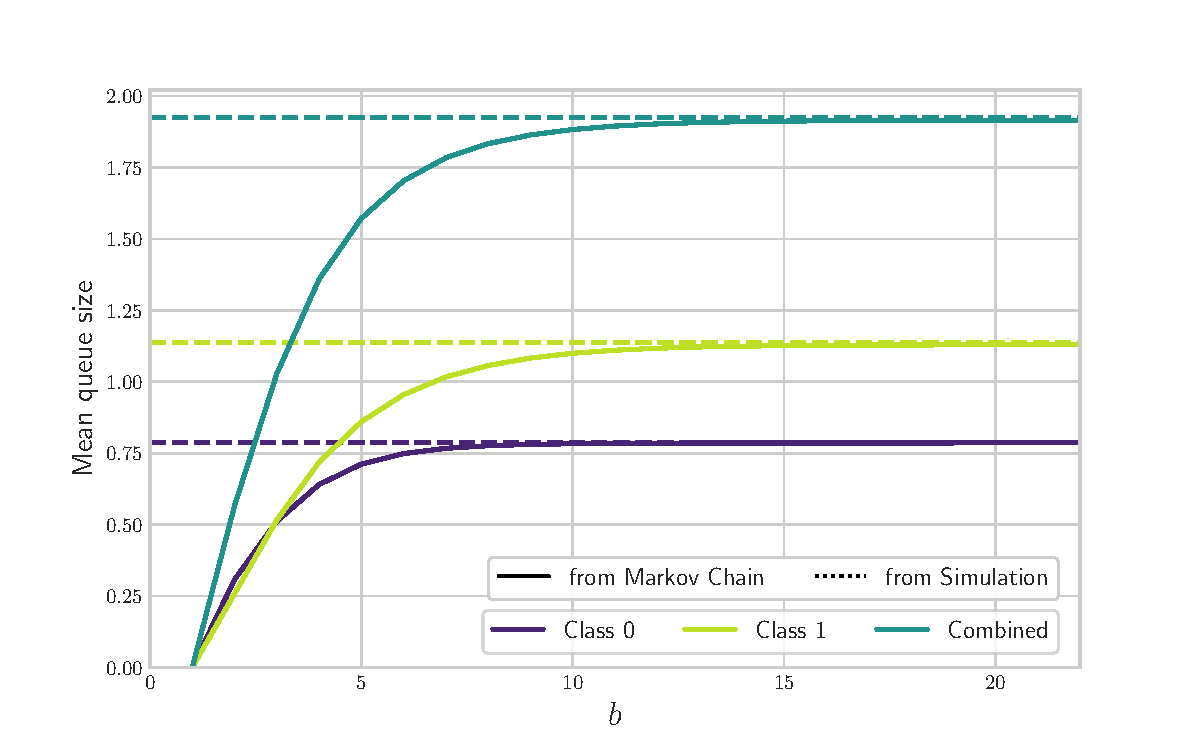
\includegraphics[width=0.6\textwidth]{img/queue_size_bound_approaches.pdf}
    \caption{Demonstrating that as $b$ increases, the expected number of
    customers of each class approaches that found using a long run simulation.}
    \label{fig:kpi_approaches_numcusts}
  \end{center}
\end{figure}

\begin{figure}
  \begin{center}
    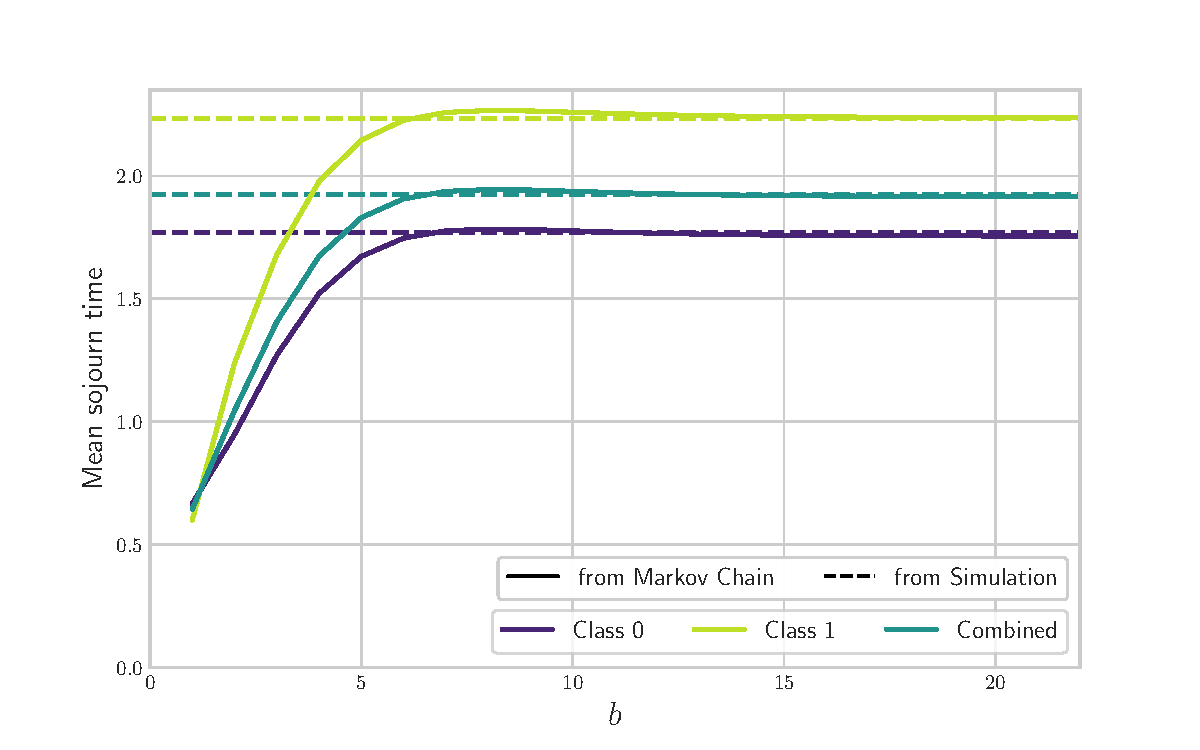
\includegraphics[width=0.6\textwidth]{img/sojourn_time_bound_approaches.pdf}
    \caption{Demonstrating that as $b$ increases, the expected sojourn time of
    customers of each class approaches that found using a long run simulation.}
    \label{fig:kpi_approaches_sojourn}
  \end{center}
\end{figure}

This is an inefficient way of determining the accuracy of the bounded
approximation. It would be more efficient to choose a $b$ and be able to
immediately measure if the accuracy is sufficient. We propose two measures, one
for the ergodic Markov chains of Section~\ref{sec:state_formulation}, and one
for the absorbing Markov chains of Section~\ref{sec:sojourn_formulation}).


\subsubsection{Accuracy measure for the ergodic Markov chain}\label{sec:ergodic_accuracy}
Let $S_b = \{\underline{\mathbf{s}} \in S \;|\; b \in \underline{\mathbf{s}}\}$,
the set of states that lie on the Markov chain boundary. We wish to choose $b$
large enough that the boundary is irrelevant, that is that the Markov chain
hardly ever reaches the boundary. Therefore we propose the \textit{relative}
probability of being at the boundary, $\mathcal{Q}(b)$, to be a measure of
accuracy; if this is sufficiently small, then the bound $b$ is large enough.
This, given in Equation~\ref{eqn:relative_probability_boundary}, is the ratio of
the probability of being at the boundary in the $b$-bounded system, and the
probability of being at the boundary if every state was equally likely. This
normalisation by the equally-likely state probabilities is necessary because the
larger $b$ is, the larger the state space is, meaning that the steady state
probabilities are spread over more states and so are not comparable alone,
whereas the relative probability of being at the boundary is comparable over
different sizes of $b$.

\begin{equation}\label{eqn:relative_probability_boundary}
\mathcal{Q}(b) = \frac{|S|}{|S_b|} \sum_{s \in S_b} \tilde{\pi}_s
\end{equation}

To demonstrate the effect of $b$ on $\mathcal{Q}(b)$ under different systems,
consider the stochastic priority switching system with two customer classes,
$\lambda_1 = \frac{1}{2}$, $\lambda_2 = \frac{1}{2}$, $c = 1$,
$\mu_1 = \frac{1}{\rho}$, $\mu_2 = \frac{1}{\rho}$, $\theta_{12} = 1$, and
$\theta_{21} = 1$; where $0 < \rho < 1$ is some given traffic intensity.
Figure~\ref{fig:ergodic_accuracy} shows the effect of $b$ on $\mathcal{Q}(b)$
for this system, for different values of $\rho$. In all cases as $b$ increases,
$\mathcal{Q}(b)$ decreases, indicating greater accuracy of the bounded system.
As expected, as $\rho$ increases, we expect more customers in the queue, and so
the boundary $b$ needs to be much larger before it can be considered irrelevant.

\begin{figure}
  \begin{center}
    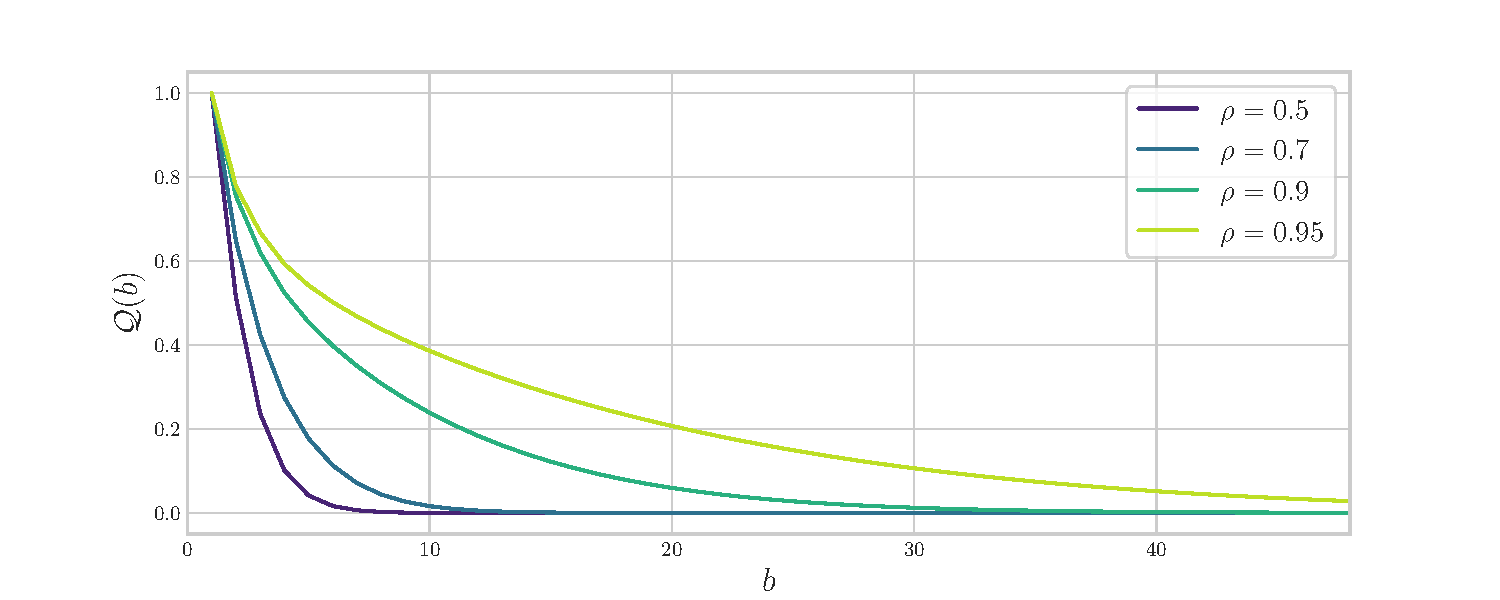
\includegraphics[width=0.8\textwidth]{img/quotient_accuracy.pdf}
  \end{center}
  \caption{Demonstration of the effect of $b$ on $\mathcal{Q}(b)$}
  \label{fig:ergodic_accuracy}
\end{figure}



\subsubsection{Accuracy measure for the absorbing Markov chain}\label{sec:absorbing_accuracy}
The above measure cannot be used for absorbing Markov chains as they will not
reach steady state, so another check is required. Define $h_{i,J}$ as the
hitting probabilities of a set of states $J$ from state $i$, that is, what is
the probability of ever reaching any state in $J$ when starting from state $i$.
These are defined recursively by Equation~\ref{eqn:hitting_probs}
\cite{privault13}, where $q_{i,k}$ is the transition rate from state $i$ to
state $j$ defined in Equation~\ref{eqn:transitions_sojourn}.

\begin{equation}\label{eqn:hitting_probs}
h_{i,J} = \begin{cases}
\sum_k q_{i,k} h_{k,J} & \text{if } i \notin J \\
1 & \text{if } i \in J
\end{cases}
\end{equation}

Relating this to the absorbing Markov chain described in
Section~\ref{sec:sojourn_formulation}, and letting $Z_b \subset Z$ be the set of
boundary states such that
$Z_b = \{\underline{\mathbf{z}} \in Z \; | \; b \in \underline{\mathbf{z}}\}$,
then if a customer arrives to state $i$, the probability of that customer's
state reaching the boundary is $h_{i,S_b}$. Therefore we propose the probability
of an arriving customer experiencing the boundary, $\mathcal{P}(b)$, to be a
measure of accuracy; if this is sufficiently small, then the bound $b$ is large
enough. This is calculated in a similar way to the mean sojourn time in
Section~\ref{sec:meansojourncalc}, and given in Equation~\ref{eqn:hitting_measure}.

\begin{equation}\label{eqn:hitting_measure}
\mathcal{P}(b) = \sum_{\underline{\mathbf{z}} \in \tilde{Z}} \sum_{k=0}^{K-1} \frac{\lambda_k}{\sum_{i=0}^{K-1} \lambda_i} \pi_{c(\underline{\mathbf{z}})} h_{\underline{\mathbf{z}}, Z_b}
\end{equation}

To demonstrate the effect of $b$ on $\mathcal{P}(b)$ under different system,
consider the same stochastic priority switching system with two customer classes
used in the previous demonstration. Figure~\ref{fig:hitting_accuracy} shows the
effect of $b$ on $\mathcal{P}(b)$ for this system, for different values of $\rho$.
Again, in all cases as $b$ increases, $\mathcal{P}(b)$ decreases, indicating
greater accuracy of the bounded system; and similarly as $\rho$ increases the
boundary $b$ needs to be larger before it can be considered irrelevant.

\begin{figure}
  \begin{center}
    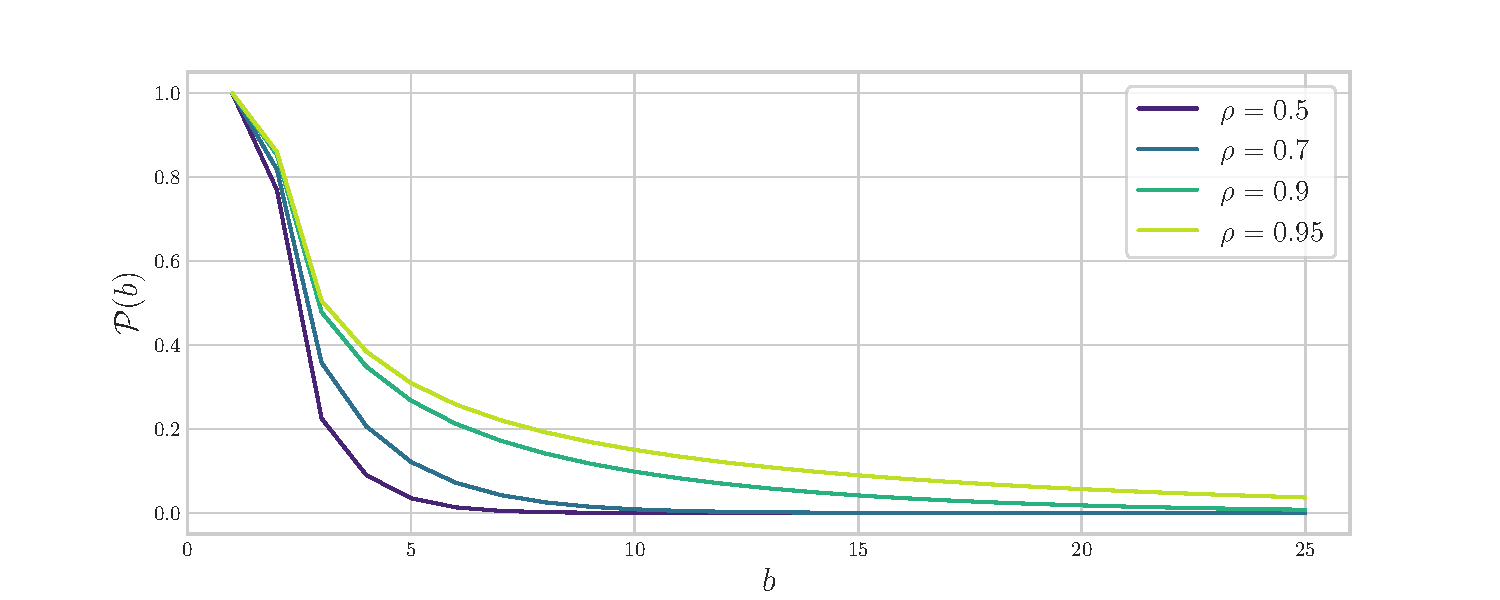
\includegraphics[width=0.8\textwidth]{img/hitting_accuracy.pdf}
  \end{center}
  \caption{Demonstration of the effect of $b$ on $\mathcal{P}(b)$}
  \label{fig:hitting_accuracy}
\end{figure}

Appendix~\ref{apx:more_priority_classes} shows examples where the simulation and
Markov chains given the state probabilities, for $K = 2$, $K = 3$, and $K = 4$
priority classes.

\subsection{Existence of Stationary Distributions}\label{sec:stationary}
In all cases, the $b$-bounded system will only be an approximation of the
infinite system of that infinite system is stationary, that is it reaches a
steady-state and the queue does not grow indefinitely.
Proposition~\ref{thrm:steadystate} gives a naive check for the existence or
non-existence of steady states for work conserving queues, but does not cover
all possibilities. A work conserving queue is one where the total work that
needs to be done by the servers is not lowered or increased by the priority or
service discipline \cite{wolff70}.

\begin{prop}\label{thrm:steadystate}
For an $M/M/c$ work conserving queue with $K$ classes of customer, with arrival
rate and service rate $\lambda_k$ and  $\mu_k$ for customers of class $k$,
respectively; then
\begin{enumerate}
  \item it will reach steady state if
  $\rho_{\max} = \frac{\sum_i \lambda_i}{c \min_i \mu_i} < 1$,
  \item it will never reach steady state if
  $\rho_{\min} = \frac{\sum_i \lambda_i}{c \max_i \mu_i} \geq 1$.
\end{enumerate}
\end{prop}

Note that this result does not assume any particular service discipline such as
first-in-first-out or stochastically changing prioritised classes, but holds for
any work conserving discipline.

\begin{proof}
The queue will reach steady state if the rate at which customers are added to
the queue is less than the rate at which customers leave the queue.
As arrivals are not state dependent, customers are added to the queue at a rate
$\sum_i \lambda_i$ when in any state.
The rate at which customers leave the queue is state dependent, depending on the
service discipline.

We do not need to consider cases when there are less than $c$ customers present,
as here any new arrival will increase the rate at which customers leave the
queue, as that arrival would enter service immediately.
Considering the cases where there are $c$ or more customers in the queue, there
are two extreme cases, either:

\begin{enumerate}
  \item all customers in service are of the class with the slowest service rate.
  In this case the rate at which customers leave the queue is $c \min_i \mu_i$,
  which is the slowest possible rate at which customers can leave the queue.
  If $\sum_i \lambda_i < c \min_i \mu_i$ then the rate at which customers enter
  the queue is smaller than the smallest possible rate at which customers leave
  the queue, and so will always be smaller than the rate at which customers
  leave the queue in all states. Therefore the system will reach steady state.
  Or:
  \item all customers in service are of the class with the fastest service rate.
  In this case the rate at which customers leave the queue is $c \max_i \mu_i$,
  which is the fastest possible rate at which customers can leave the queue.
  If $\sum_i \lambda_i \geq c \max_i \mu_i$ then the rate at which customers
  enter the queue is greater than or equal to the largest possible rate at which
  customers leave the queue, and so will always be greater or equal to than the
  rate at which customers leave the queue in all states. Therefore the system
  cannot reach steady state.
\end{enumerate}
\end{proof}

Proposition~\ref{thrm:steadystate} applies to the stochastic priority switching
system of this paper. If pre-empted customers resume their service upon
re-entering service, then the system is work conserving. Otherwise, if the
pre-empted customers restart or resample their service, despite not technically
being work conserving any more, the systems are equivalent under Exponential
service times, and so still applies here.

If $c \min_i \mu_i \leq \sum_i \lambda_i < c \max_i \mu_i$ then more
investigation is needed. In the case of stochastic priority switching, the class
change matrix $\Theta$ may be significant. For example the service rate of
customers of one class may be very slow, however if the rate at which customers
leave that class is sufficiently large then that service rate may not have an
effect. Alternatively if the rate at which customers of the other classes change
to that class is large, then that slow service rate could be a bottleneck for
the system.

We can however approximately test if a system is stationary or not using
simulation. Consider the time series $x(t)$, representing the total number of
customers in the system at time $t$. In Ciw, this can be empirically recorded
using a state tracker object. If the system reaches steady state, then the
$x(t)$ will be stochastic with non-increasing trend, therefore it would be a
stationary time series. Conversely, if the system does not reach steady state,
then $x(t)$ will be stochastic with increasing trend, therefore it would be a
non-stationary time series.
The Augmented Dicky-Fuller (ADF) test \cite{dickyfuller79} tests for the
non-stationarity of a stochastic time series, and so can be utilised here to
test if a simulation has reached steady state or not. Note here that the time
series $x(t)$ recorded by Ciw has irregular gaps (time stamps are the discrete
time points where a customer arrives or leaves the system), and the ADF test
requires regularly spaced time stamps; therefore the Traces library
\cite{traces} is used to take regularly-spaced moving averages before the
hypothesis test is undertaken.

To demonstrate this, consider two examples, with parameters defined in
Table~\ref{tbl:adf_example_parameters}. Example 1 is guaranteed to reach steady
state by Proposition~\ref{thrm:steadystate}, while Example 2 is guaranteed not
to reach steady state.

\begin{table}
\begin{center}
\begin{tabular}{rrrrrrrr}
\toprule
 & $\lambda_1$ & $\lambda_2$ & $c$ & $\mu_1$ & $\mu_2$ & $\theta_{12}$ & $\theta_{21}$ \\
\midrule
Example 1 & 2 & 1 & 1 & 4 & 4 & 1 & 1\\ 
Example 2 & 2 & 1 & 1 & 1 & 1 & 1 & 1\\ 
\bottomrule
\end{tabular}
\end{center}
\caption{Parameters used in demonstrations of the ADF test.}
\label{tbl:adf_example_parameters}
\end{table}

\begin{figure}
  \begin{center}
  \begin{subfigure}[b]{0.45\textwidth}
    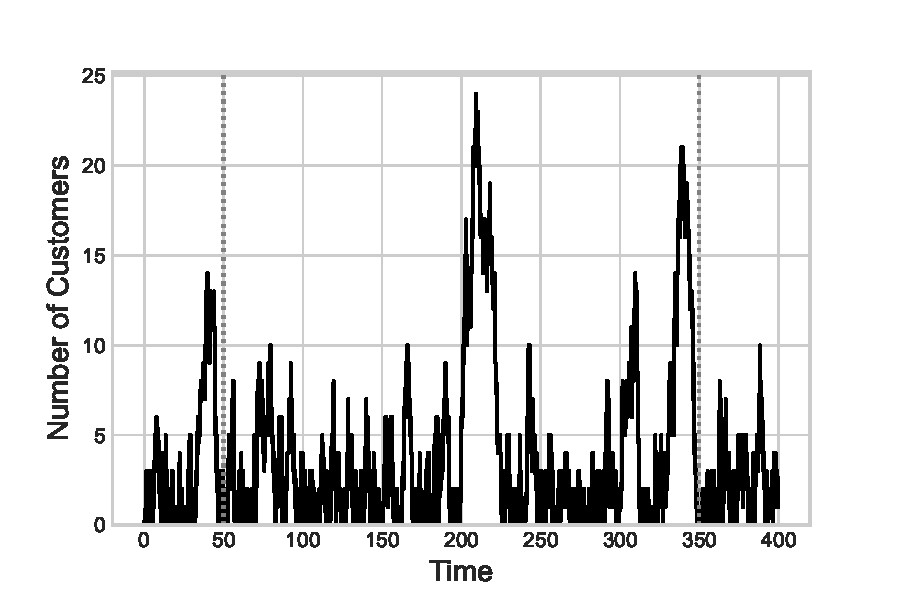
\includegraphics[width=\textwidth]{img/adf_test_steadystate.pdf}
    \caption{State time series for Example 1.}
    \label{fig:timeseries1}
  \end{subfigure}
  \begin{subfigure}[b]{0.45\textwidth}
    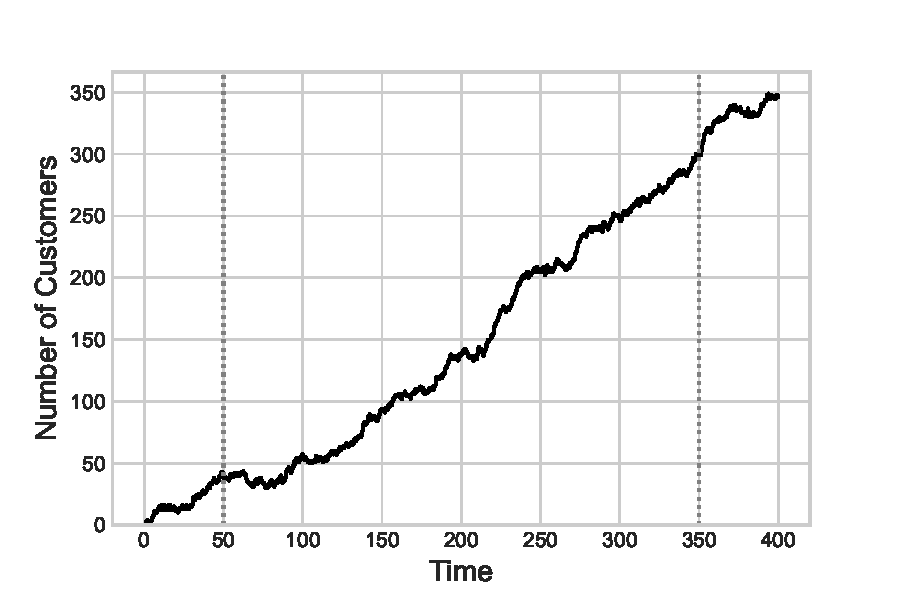
\includegraphics[width=\textwidth]{img/adf_test_not_steadystate.pdf}
    \caption{State time series for Example 2.}
    \label{fig:timeseries2}
  \end{subfigure}
  \caption{Demonstration of the ADF test on states that do and do not reach
  steady state according to Proposition~\ref{thrm:steadystate}.}
  \end{center}
\end{figure}


Figures~\ref{fig:timeseries1} and~\ref{fig:timeseries2} shows their state time
series' $x(t)$ respectively. It is clear that the state time series for
Example~1 is stationary, and the state time series for Example~2 is
non-stationary and increasing. When performing the ADF test on these, Example~1
gives a p-value of 0.0004, rejecting the null hypothesis that the time series is
non-stationary, while Example 2 gives a p-value of 0.9961, and the null
hypothesis cannot be rejected.

There is a gap in Proposition~\ref{thrm:steadystate} for systems where
$c \min_i \mu_i \leq \sum_i \lambda_i < c \max_i \mu_i$. Indeed it is in this
gap that our previous scenario in Figure~\ref{fig:toy_scenario} falls, and it is
here where stochastic priority switching can influence the stationarity of the
system. Consider a two class system with $\lambda_1 = 2$, $\lambda_2 = 2$,
$c = 1$. For the service rates of each customer class, consider two cases:

\begin{itemize}
  \item $\mu_1 = 3$ and $\mu_2 = 5$: here
  $\rho_{\text{min}} < 1 < \rho_{\text{max}}$, and the prioritised class receive
  a slower service rate;
  \item $\mu_1 = 5$ and $\mu_2 = 3$: here
  $\rho_{\text{min}} < 1 < \rho_{\text{max}}$, and the prioritised class receive
  a faster service rate.
\end{itemize}

In each of these cases, we can consider three other cases pertaining to the
class change rate matrix $\Theta$:

\begin{itemize}
  \item $\theta_{12} = 1$ and $\theta_{21} = 0$: downgrades but no upgrades;
  \item $\theta_{12} = 1$ and $\theta_{21} = 1$: both downgrades and upgrades;
  \item $\theta_{12} = 0$ and $\theta_{21} = 1$: upgrades but no upgrades.
\end{itemize}

All these cases are not covered by Proposition~\ref{thrm:steadystate}, so we
experimentally investigate their stationarity using the Ciw simulation and ADF
test. Figure~\ref{fig:adf_gap} shows the results. Here we see that three of the
six cases are stationary, (a), (e), and (f), while the others are not. In all
three we see that there is possibility of a customer from the class with the
slower service rate transitioning to a class with the quicker service rate. In
two of the non-stationary cases, (c) and (d), customers with the slower service
rate have no possibility of transitioning out of their class, and so the queue
builds up indefinitely.
It is interesting to compare cases (b) and (e), in which both customer classes
can transition to the other customer class. Here one case is stationary, and the
other is non-stationary, with the only difference being whether the prioritised
class has the quicker service rate or not. This evidences the interesting
interplay between service rate, priority class, and class change rates.

\begin{figure}
  \begin{center}
    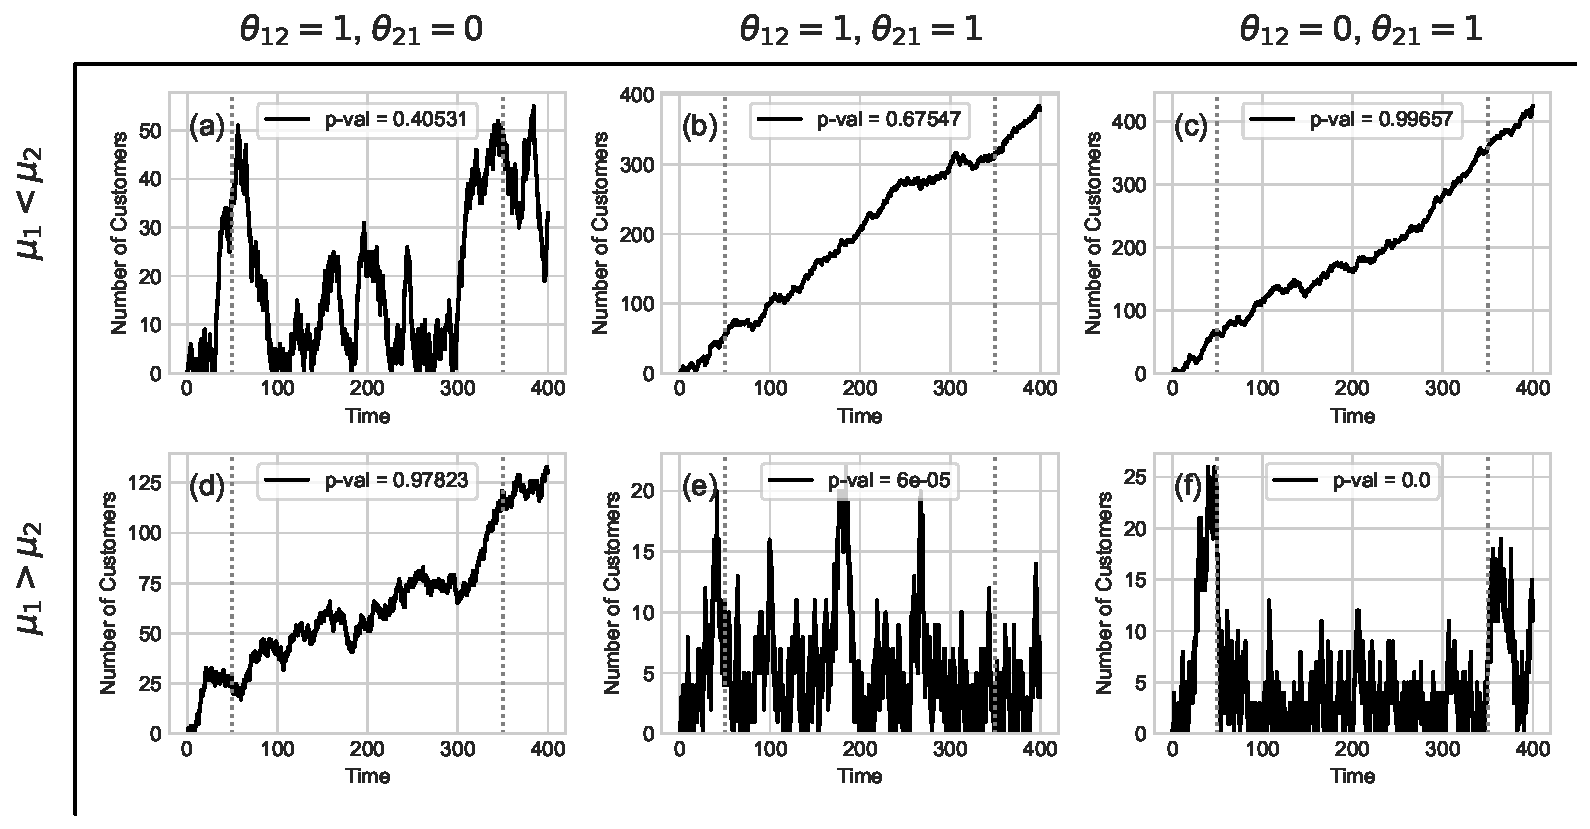
\includegraphics[width=\textwidth]{img/adf_theorem_gap.pdf}
    \caption{Investigating the stationarity under six cases not covered by
    Proposition~\ref{thrm:steadystate}.}
    \label{fig:adf_gap}
  \end{center}
\end{figure}



\subsection{Effect of $\Theta$ on Customer Experience}\label{sec:behaviour}
In Section~\ref{sec:modelling} that it is established that some service
disciplines can be modelled as stochastically changing priorities with a class
change matrix $\Theta$, and we now have Markov chain models that can be used to
consider the effect of $\Theta$ on the system behaviour. We now investigate the
effect of this matrix on customer experience, as this would be important for the
modelling process, and also for controllers of the system who might be able to
influence the rates and improve customer experience or system outcomes.

We first define two scenarios that we will use to investigate the effect of
$\Theta$, defined in Table~\ref{tbl:scenarios}. Both scenarios involve two
classes of customer, in Scenario A prioritised customers have a slower service
rate than unprioritised customer, while in Scenario B prioritised customers have
a faster service rate than prioritised customers. The Markov chain models of
Section~\ref{sec:makovchains} are built with these parameters, and all values
of $\theta_{12}$ and $\theta_{21}$ ranging from 0 to 3, in steps of 0.2, with a
bound of 16 (all producing accuracy measures
$\mathcal{Q}(16), \mathcal{P}(16) < 0.012$),
and customer experience statistic are found and compared.

\begin{table}
\begin{center}
\begin{tabular}{rrrrrr}
\toprule
Scenario & $\lambda_1$ & $\lambda_2$ & $c$ & $\mu_1$ & $\mu_2$ \\
\midrule
A & 1 & 1 & 1& $\sfrac{5}{2}$ & $\sfrac{7}{2}$\\ 
B & 1 & 1 & 1& $\sfrac{7}{2}$ & $\sfrac{5}{2}$\\
\bottomrule
\end{tabular}
\end{center}
\caption{Parameters used in experiments that investigate the effect of $\Theta$.}
\label{tbl:scenarios}
\end{table}

Figures~\ref{fig:meancusts_A} and~\ref{fig:meancusts_B} give $L_1$ and $L_2$,
the steady-state average number of customers of each class, for all pairs of
$\theta_{12}$ and $\theta_{21}$, under Scenarios A and B respectively. In
general it can be seen that as $\theta_{12}$ increases in comparison to
$\theta_{21}$ then we expect less customers of class 1 and more of class 2, and
the opposite is true as $\theta_{21}$ increases in comparison to $\theta_{12}$.
At first it seems that when $\theta_{12} \approx \theta_{21}$ the magnitude of
the rate does not have a big effect of the number of customers of each class
present, however further investigation shows this not to be the case.
Figure~\ref{fig:theta_magnitude} shows the mean number of class 1 and class 2
customers when $\theta_{12} = \theta_{21} = \tilde{\theta}$, under Scenarios A
and B, as the magnitude $\tilde{\theta}$ changes. In Scenario A, where
prioritised customers have a slower service rate, increasing the priority change
rate increases the prioritised customers present, and decreases the number of
unprioritised customers. In Scenario B the opposite trend is true. Looking at
the effect of $\tilde{\theta}$ on the overall number of customers present, in
Figure~\ref{fig:theta_magnitude_overall} we see that a higher rate of priority
changes increases the number of customers in Scenario A, but decreases the
number of customers in Scenario B. This may be because as the rate of priority
changes increases, each customer is more likely to be served as a prioritised
customer, and in Scenario B prioritised customers are processed quicker.

\begin{figure}
  \begin{center}
  \begin{subfigure}[b]{0.49\textwidth}
    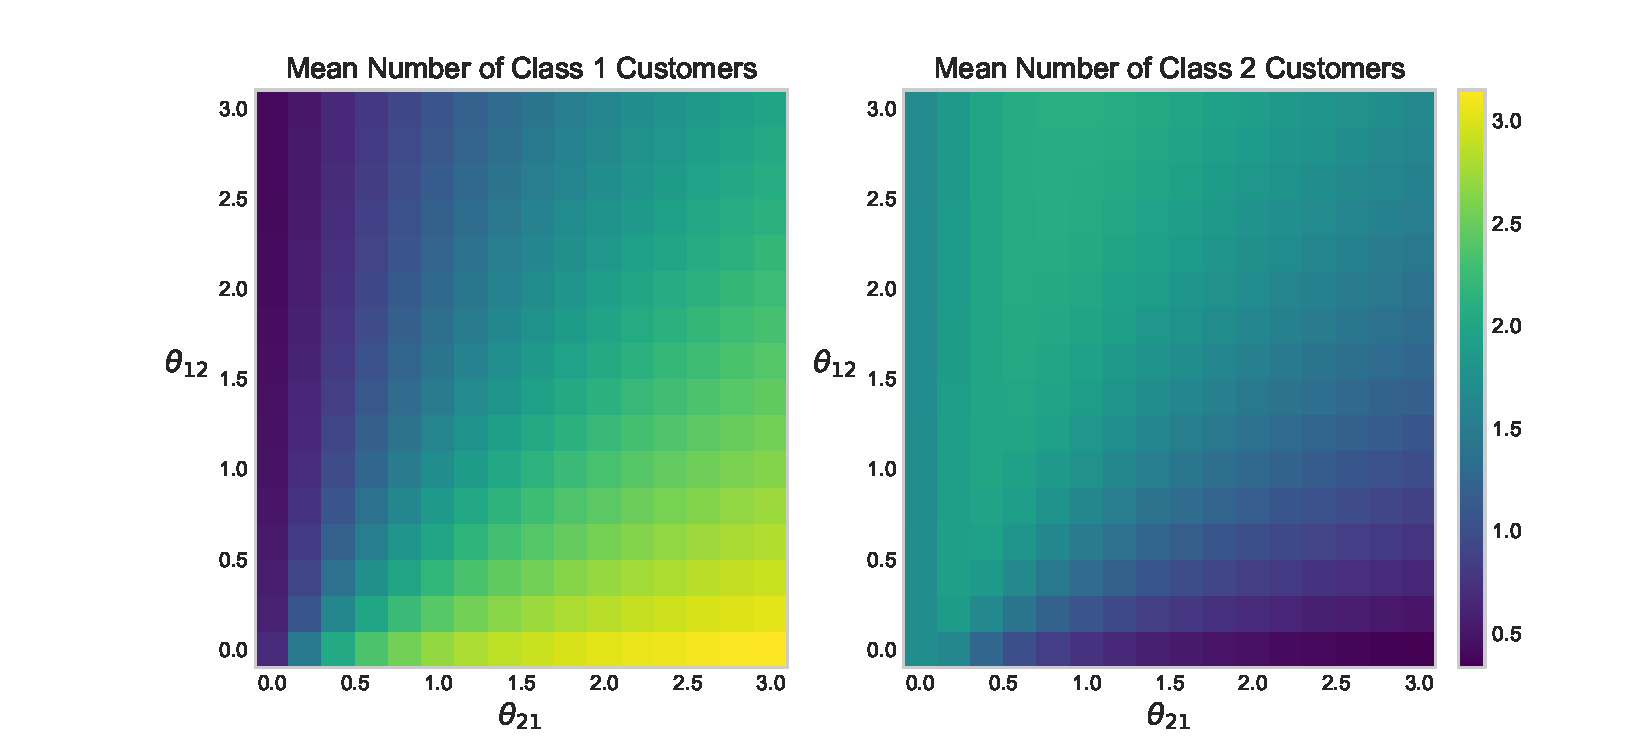
\includegraphics[width=\textwidth]{img/vary_thetas_meancusts_scen1.pdf}
    \caption{Scenario A.}
    \label{fig:meancusts_A}
  \end{subfigure}
  \begin{subfigure}[b]{0.49\textwidth}
    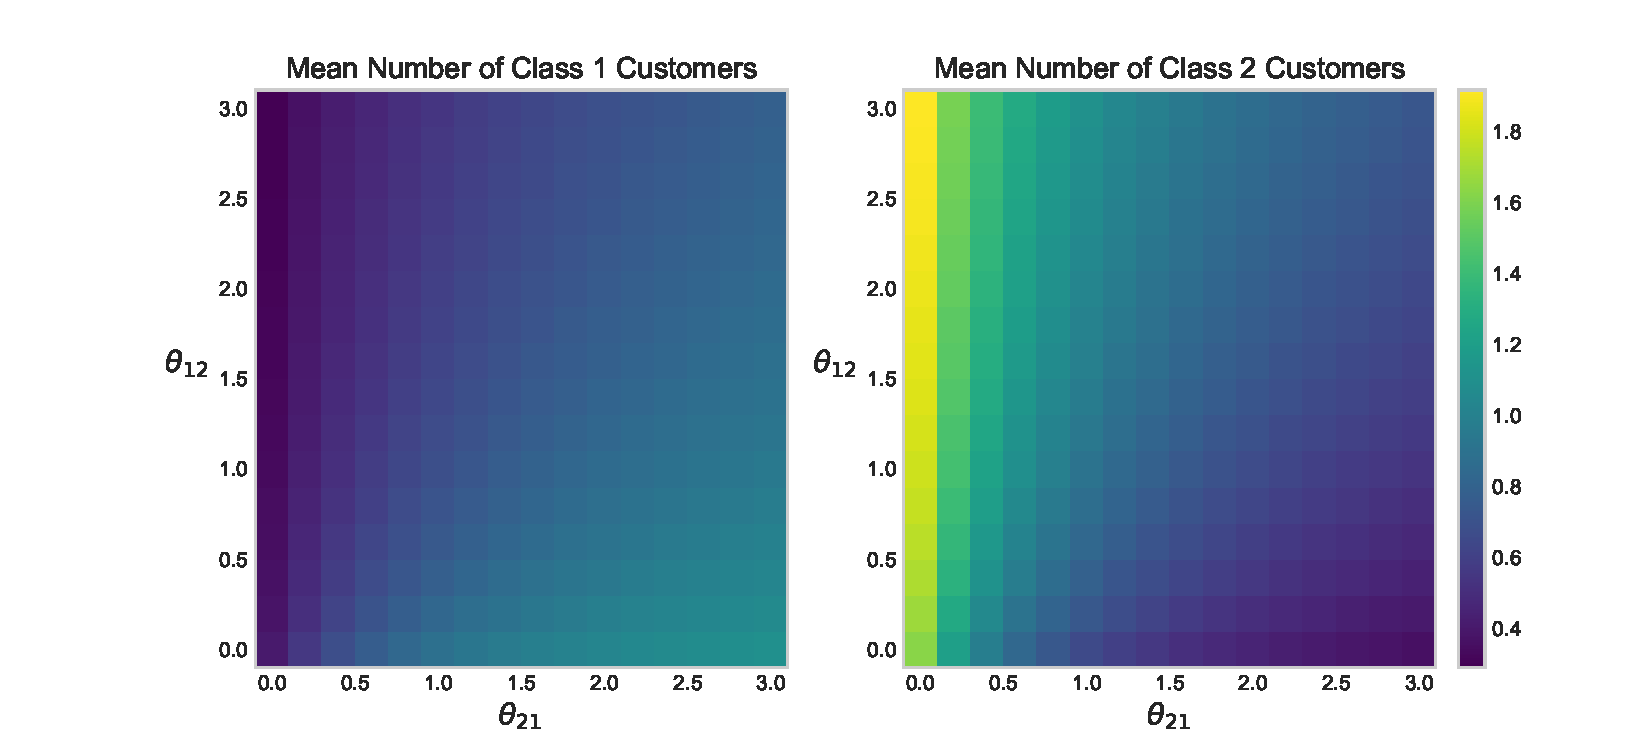
\includegraphics[width=\textwidth]{img/vary_thetas_meancusts_scen2.pdf}
    \caption{Scenario B.}
    \label{fig:meancusts_B}
  \end{subfigure}
  \caption{Average number of customers of each class, as $\Theta$ changes.}
  \end{center}
\end{figure}

\begin{figure}
  \begin{center}
    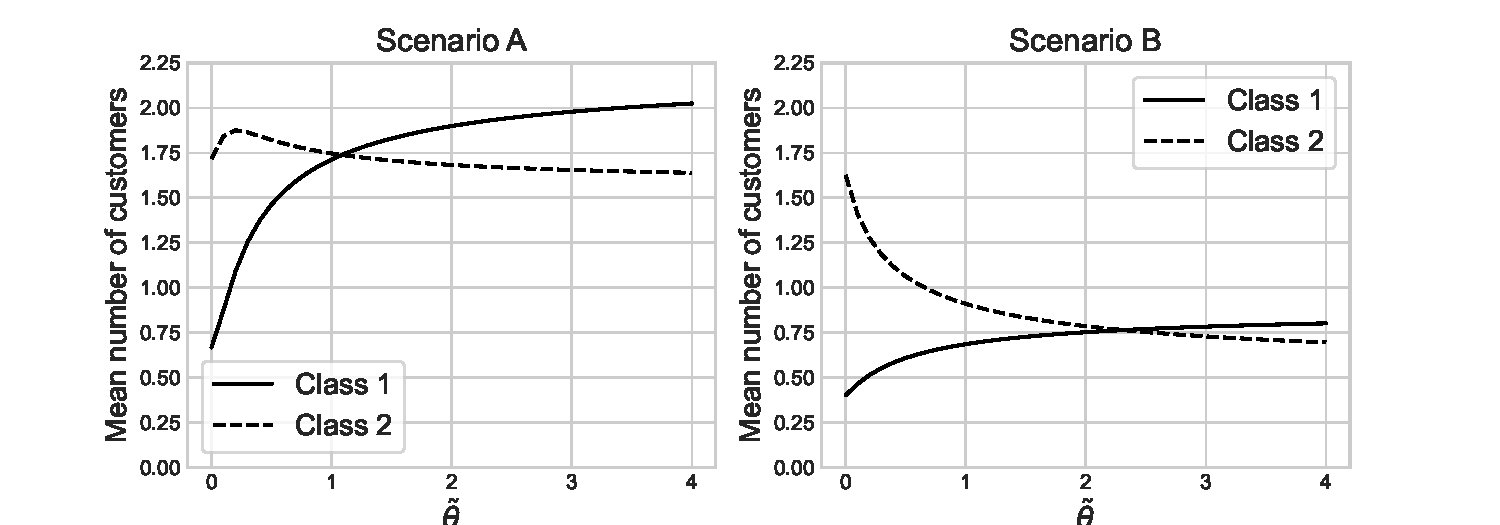
\includegraphics[width=0.7\textwidth]{img/mean_custs_equal_theta.pdf}
  \end{center}
  \caption{Average number of customers of each class, as $\tilde{\theta}$
  changes.}
  \label{fig:theta_magnitude}
\end{figure}

\begin{figure}
  \begin{center}
    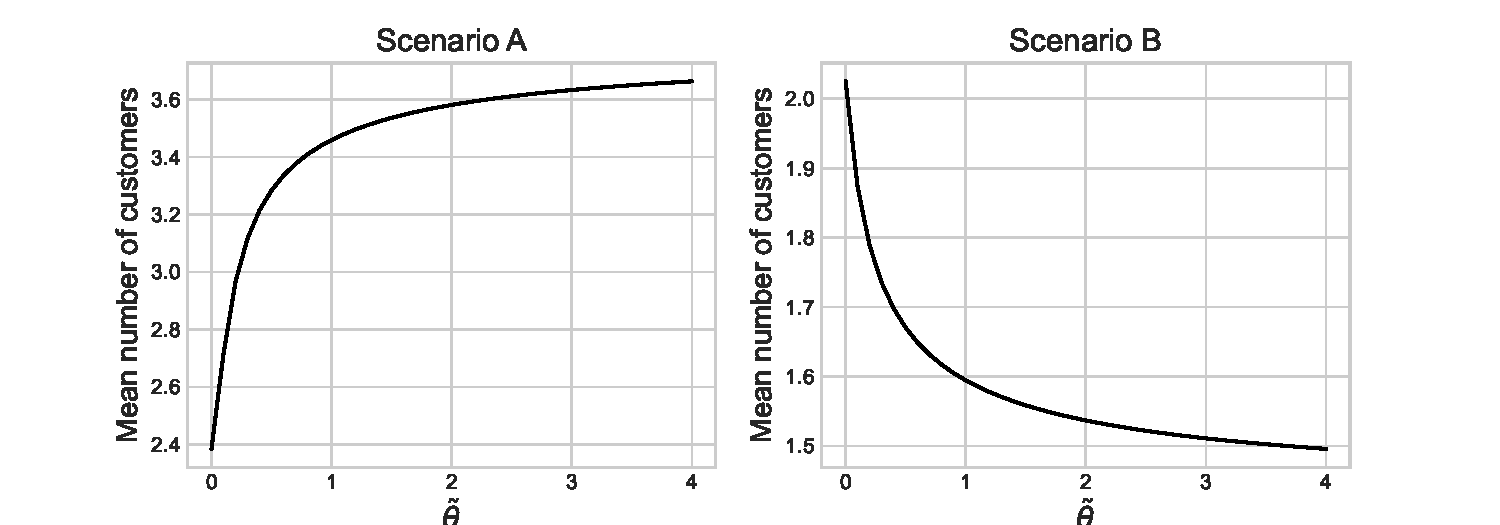
\includegraphics[width=0.7\textwidth]{img/mean_custs_equal_theta_overall.pdf}
  \end{center}
  \caption{Average number of customers overall as $\tilde{\theta}$ changes.}
  \label{fig:theta_magnitude_overall}
\end{figure}

Figures~\ref{fig:sojourn_A} and~\ref{fig:sojourn_B} give $\Psi_1$ and $\Psi_2$,
the steady-state average sojourn time of customers beginning in each class, for
all pairs of $\theta_{12}$ and $\theta_{21}$, under Scenarios A and B
respectively. The mean sojourn time for class 1 customers are hardly effected by
the size of $\theta_{12}$, but is more effected by the size of $\theta_{21}$,
likely due to an increased number of class 1 customers present when they join
the queue. The effect of $\theta_{21}$ on the mean sojourn time of class 2
customers depends on the scenario: in Scenario A the higher $\theta_{21}$, the
more likely a class 2 customer is to be served as a class 1 customer, that with
the slower service rate, and so a longer sojourn time; while in Scenario B they
are more likely to be served as a class 1 customer with higher service rate, and
so shorter sojourn time.

\begin{figure}
  \begin{center}
  \begin{subfigure}[b]{0.49\textwidth}
    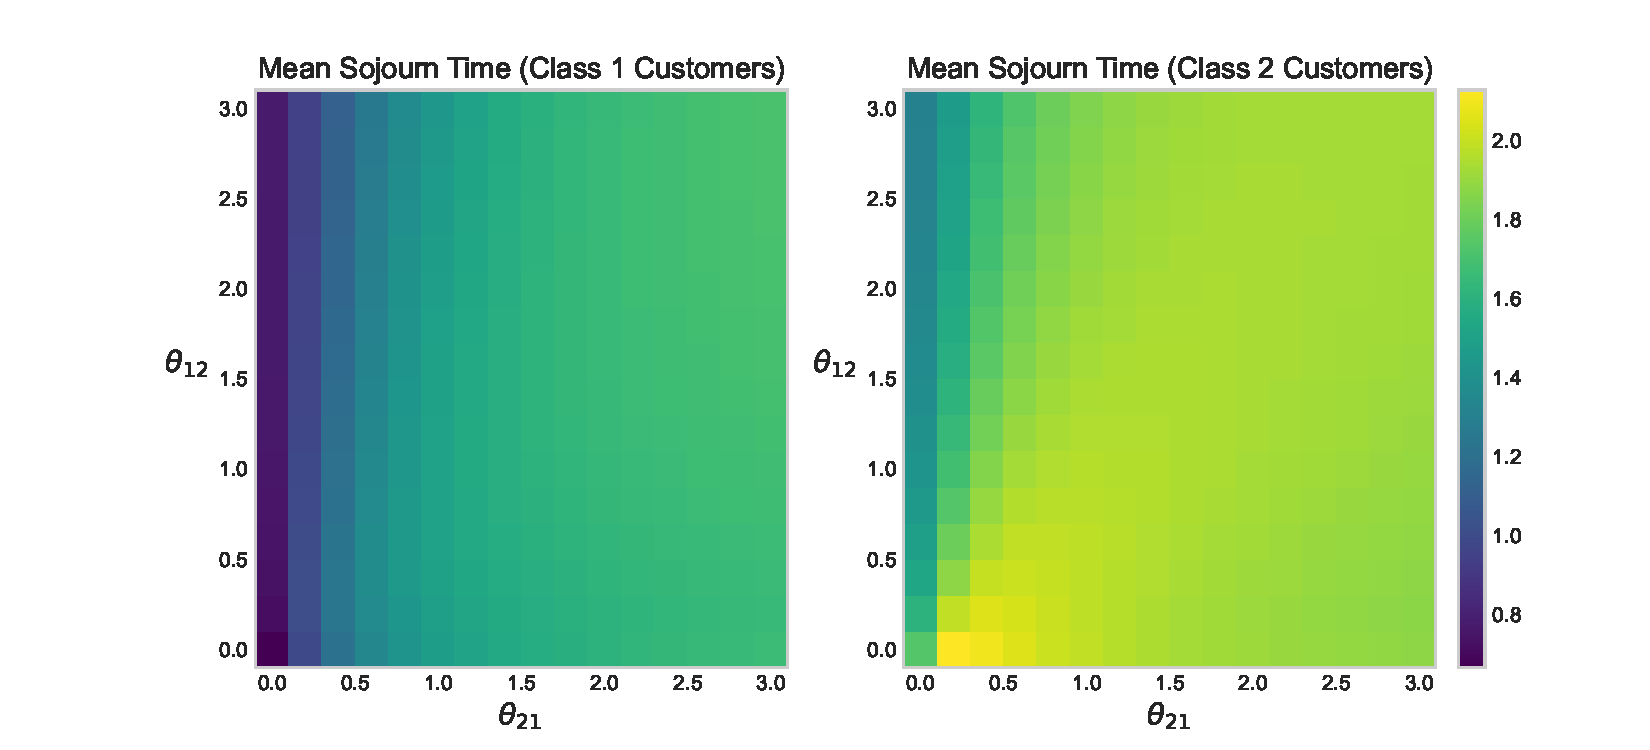
\includegraphics[width=\textwidth]{img/vary_thetas_sojourn_scen1.pdf}
    \caption{Scenario A.}
    \label{fig:sojourn_A}
  \end{subfigure}
  \begin{subfigure}[b]{0.49\textwidth}
    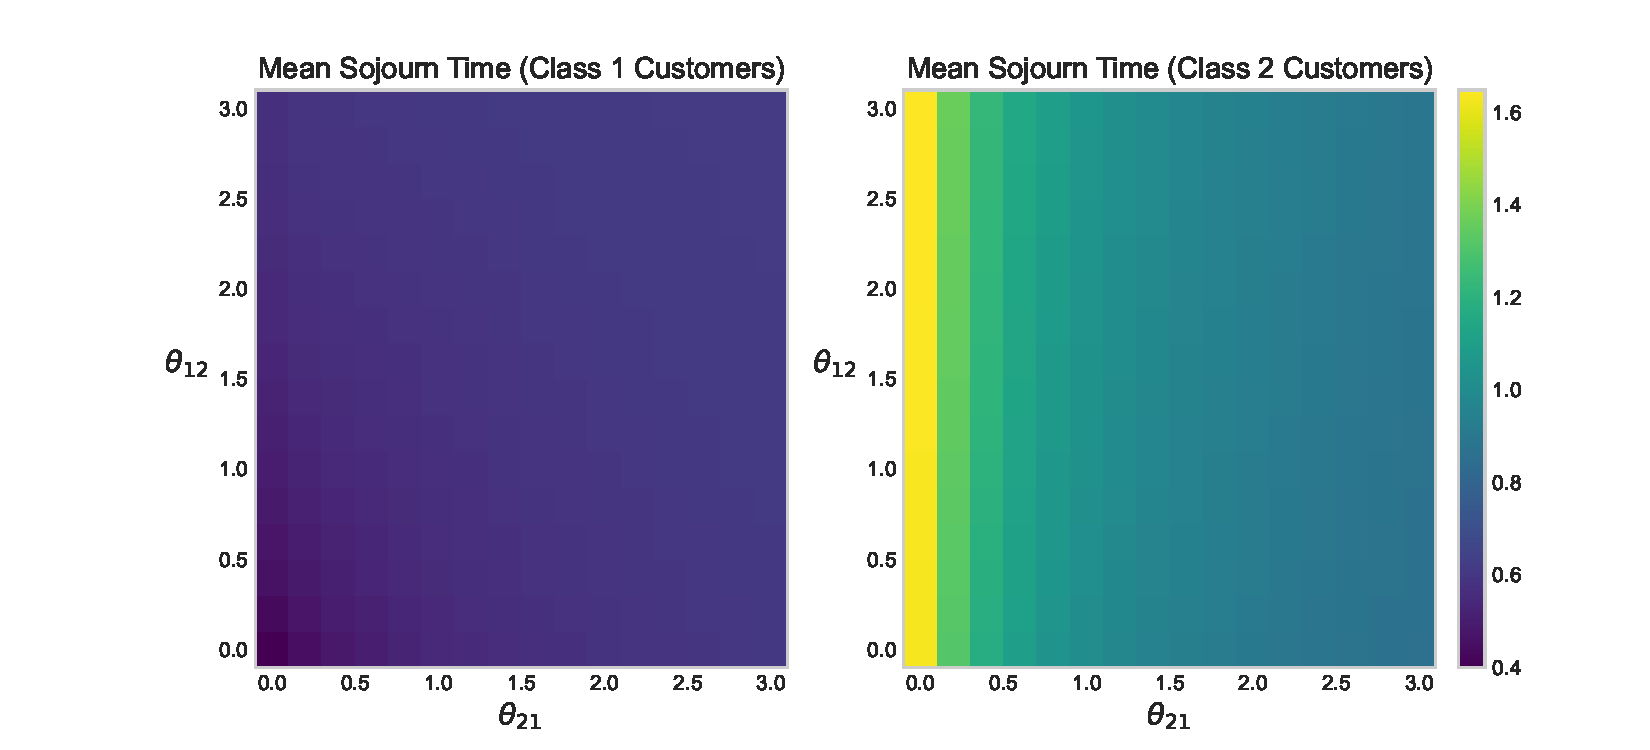
\includegraphics[width=\textwidth]{img/vary_thetas_sojourn_scen2.pdf}
    \caption{Scenario B.}
    \label{fig:sojourn_B}
  \end{subfigure}
  \caption{Average sojourn time for customers beginning in each class, as
  $\Theta$ changes.}
  \end{center}
\end{figure}


\section{Conclusions}
In this paper a generalised model of stochastic priority switching within an
$M/M/c$ queue is presented. The general formulation was given in
Section~\ref{sec:system}, followed by two methodologies for modelling it,
first by simulation, with contributions to the Ciw library, and second by two
separate Markov chains used in conjunction to find state probabilities and
customer sojourn times. In order to use the Markov chains we present bounded
approximations, and importantly we introduce two accuracy measures to
immediately determine how well the bounded Markov chain approximates its
infinite version: $\mathcal{Q}(b)$ the relative probability steady state
probability of being at the boundary, and $\mathcal{P}(b)$ the probability of an
arriving customer experiencing the boundary.

This work is motivated by modelling a healthcare situation, a surgical endoscopy
waiting list, where modelling as FIFO was inappropriate. We show that modelling
as stochastically changing priorities can approximate the queue behaviour,
with a sufficient choice of class change rate matrix $\Theta$. We then explore
the effect of this matrix on customer experience, namely mean number of
customers of each priority in the system, and mean sojourn time for each
customer class. This exploration may be useful to queue controllers, such as
waiting list managers, who can influence or tweak the class change matrix, for
example if prioritised customers have a faster service rate, then the queue is
managed better when the priority change rate is higher, though at the expense of
the prioritised customers themselves.

Although much of the work in this paper concentrated on two classes of customer
and two prioritisation levels, the formulation is generalised to any number of
customer classes, offering greater flexibility in modelling unknown service
disciplines. Similarly, the simulation methodology, implemented and available
out-of-the-box in an open-source Python package, is generalised and can model
non-Markovian priority changes too. For example a deterministic distribution,
that is one that samples the same number each time, is equivalent to a time
cut-off for priority changes.

All code and computational work used to produce this paper is openly available
at \url{https://github.com/geraintpalmer/DynamicClasses}.

\bibliographystyle{plain}
\bibliography{refs}

\newpage
\appendix

\section{Further Experiments}\label{apx:more_priority_classes}

\begin{figure}[h!]
  \begin{center}
  \begin{subfigure}[b]{\textwidth}
    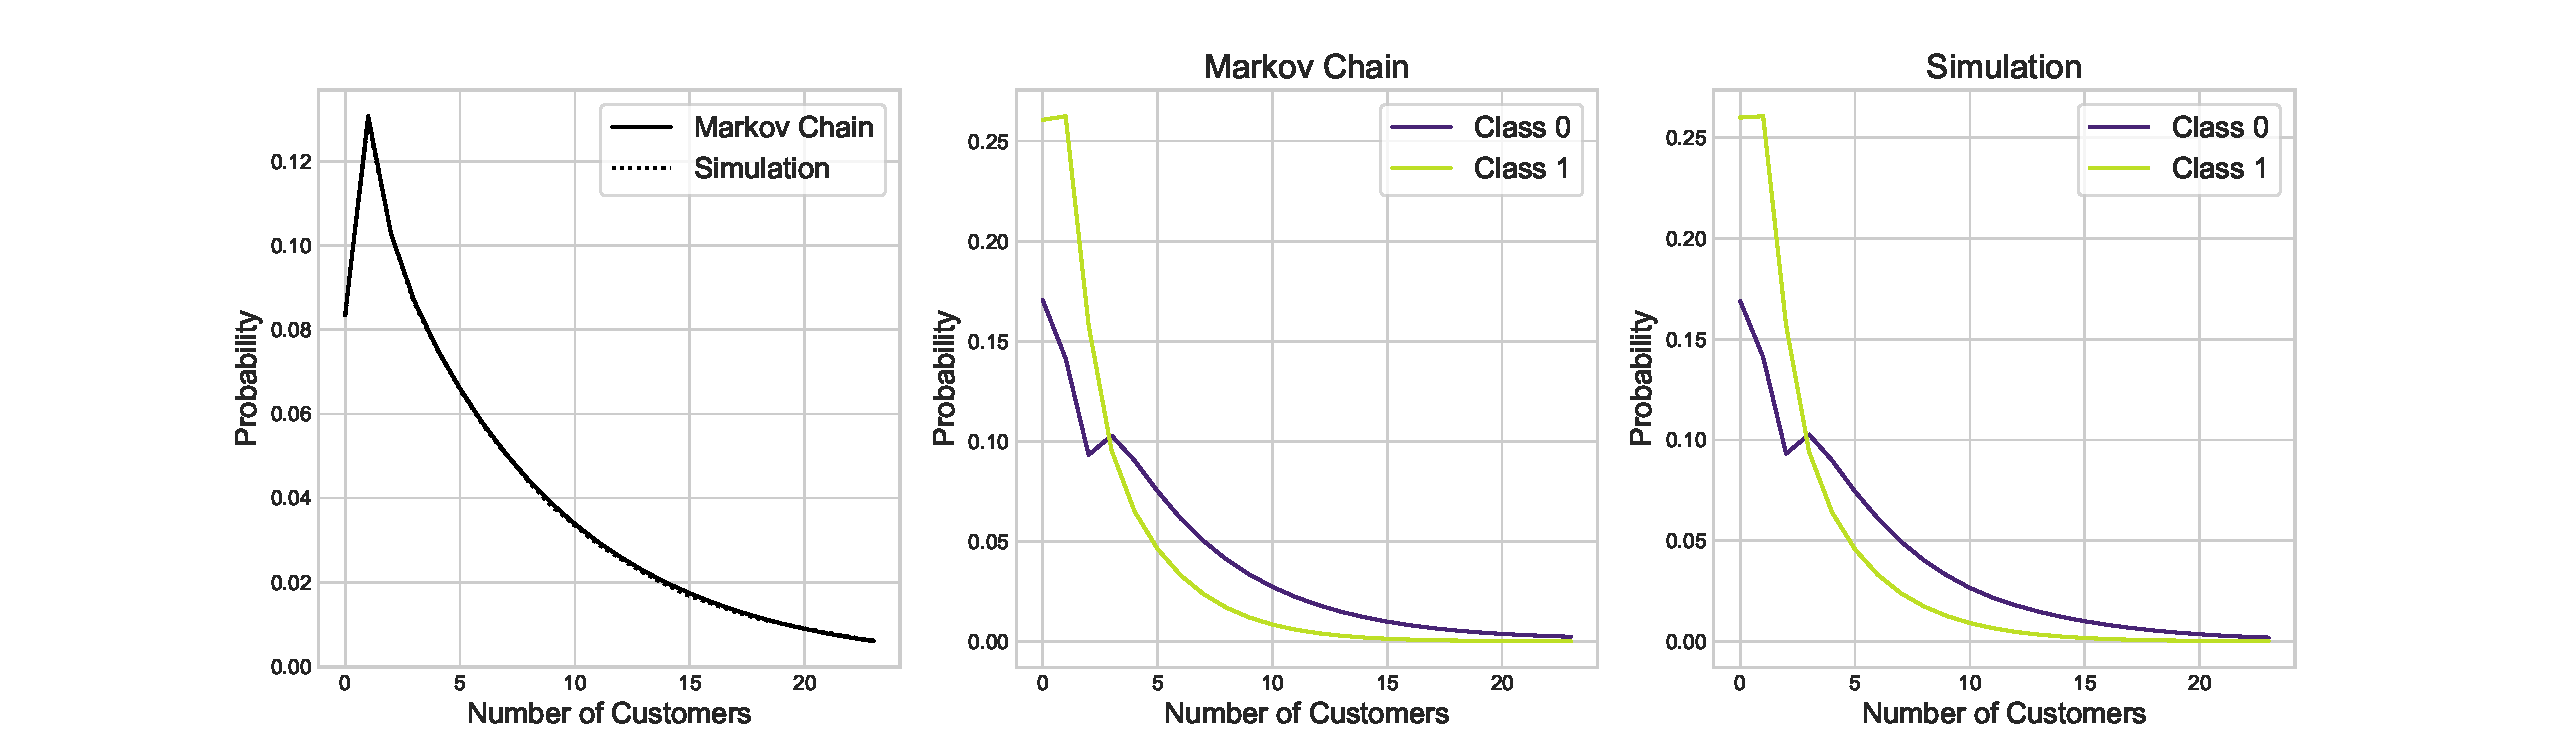
\includegraphics[width=\textwidth]{img/appendix_2class.pdf}
    \caption{
        $K = 2$
        $\begin{array}{c}\lambda_1 = 3\\\lambda_2 = 4\end{array}$
        $\begin{array}{c}\mu_1 = 4\\\mu_2 = 5\end{array}$
        $\begin{array}{c}c=2\\b=24\end{array}$
        $\Theta = \begin{pmatrix}0 & 7\\12 & 0\end{pmatrix}$
        $\begin{array}{c}\text{Simulation time} = 200000\\\text{warm-up} = 5000\end{array}$
    }
  \end{subfigure}
  \vspace{3mm}
  \begin{subfigure}[b]{\textwidth}
    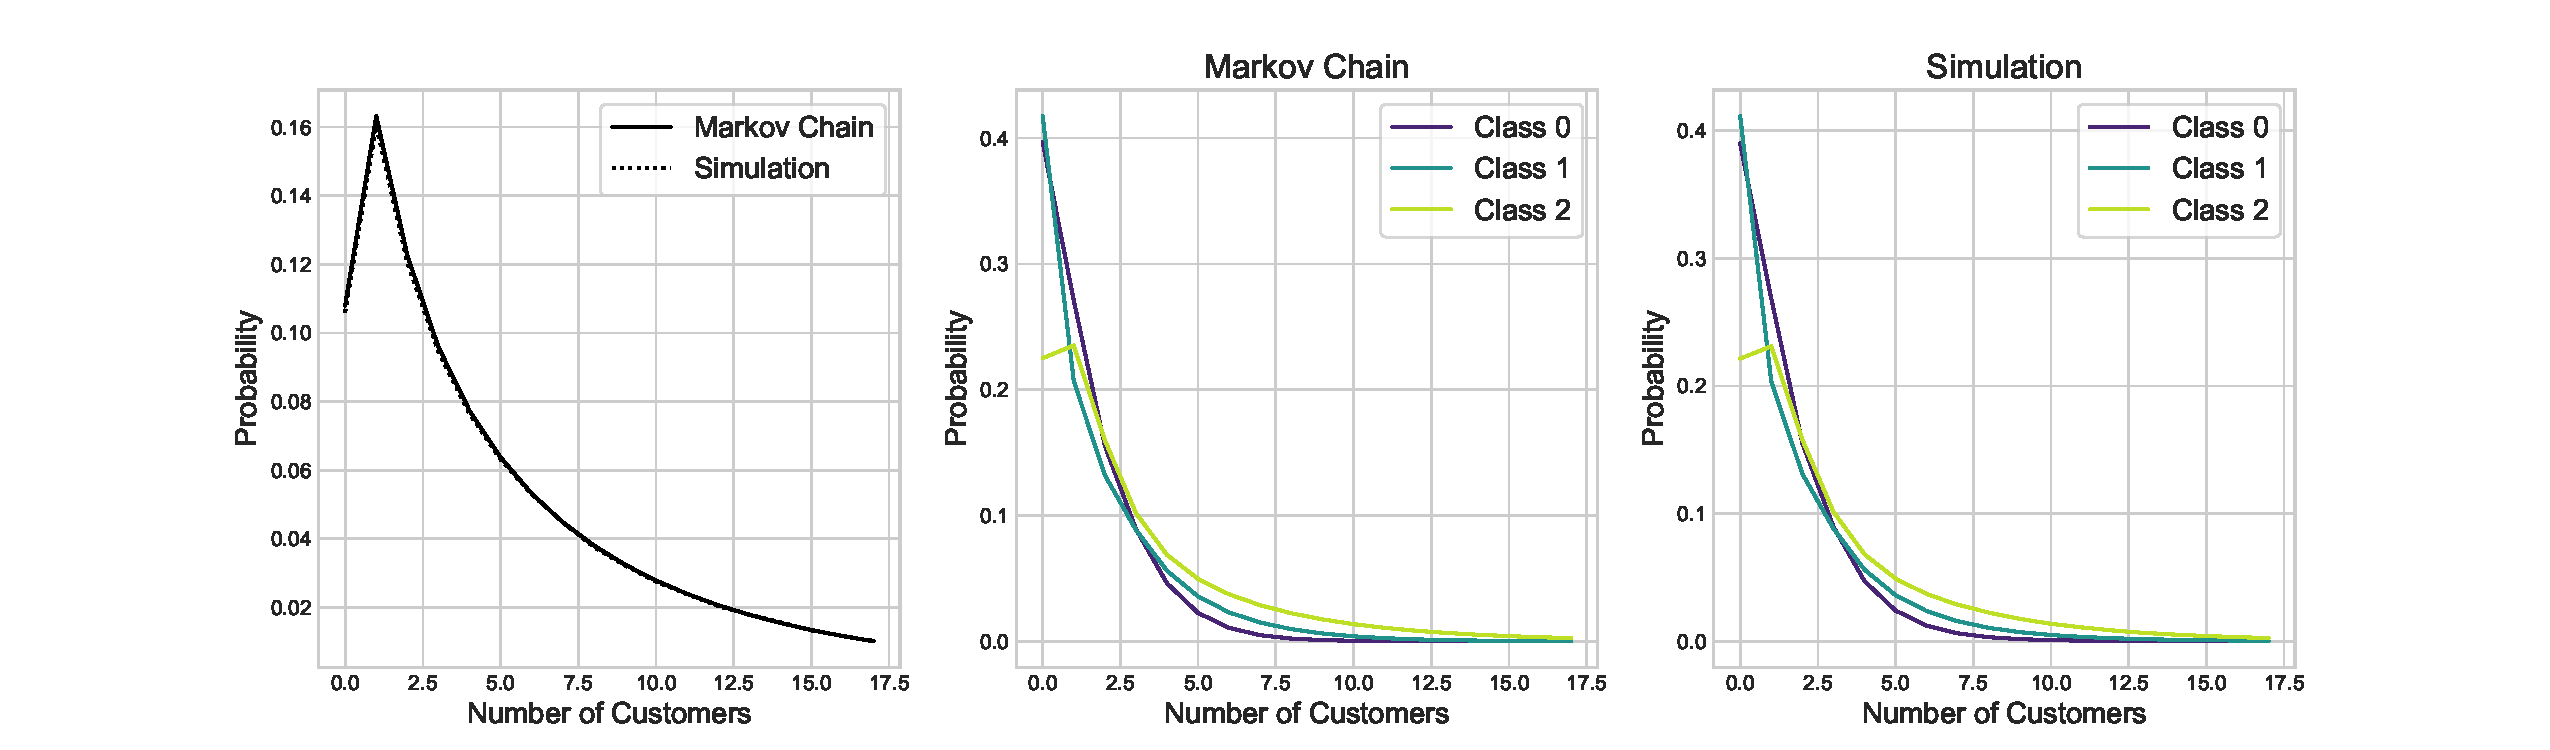
\includegraphics[width=\textwidth]{img/appendix_3class.pdf}
    \caption{
        $K = 3$
        $\begin{array}{c}\lambda_1 = 2\\\lambda_2 = 1\\\lambda_3 = 4\end{array}$
        $\begin{array}{c}\mu_1 = 4\\\mu_2 = 4.5\\\mu_3 = 5\end{array}$
        $\begin{array}{c}c=2\\b=18\end{array}$
        $\Theta = \begin{pmatrix}0 & 2 & 4\\1 & 0 & 5\\1 & 3 & 0\end{pmatrix}$
        $\begin{array}{c}\text{Simulation time} = 200000\\\text{warm-up} = 5000\end{array}$
    }
  \end{subfigure}
  \vspace{3mm}
  \begin{subfigure}[b]{\textwidth}
    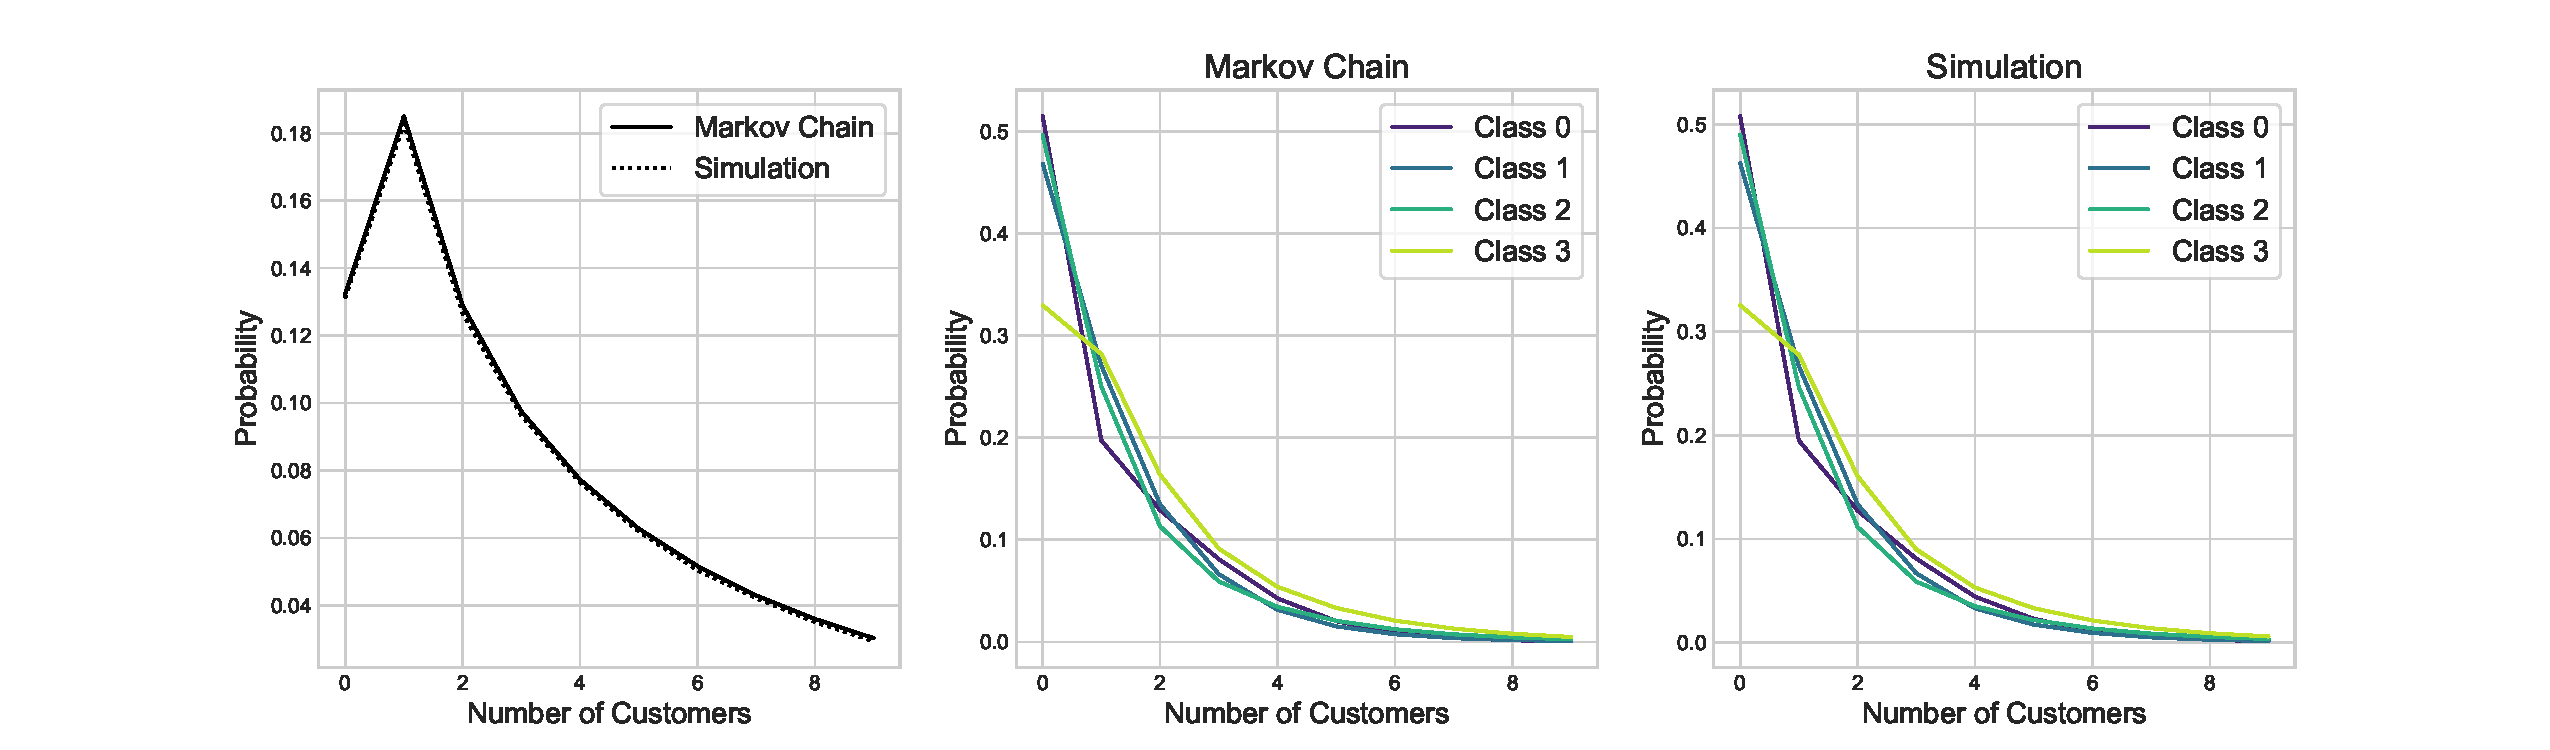
\includegraphics[width=\textwidth]{img/appendix_4class.pdf}
    \caption{
        $K = 4$
        $\begin{array}{c}\lambda_1 = 0.5\\\lambda_2 = 1.5\\\lambda_3 = 1\\\lambda_4 = 3\end{array}$
        $\begin{array}{c}\mu_1 = 3.5\\\mu_2 = 4\\\mu_3 = 3.5\\\mu_4 = 5\end{array}$
        $\begin{array}{c}c=2\\b=10\end{array}$
        $\Theta = \begin{pmatrix}0 & 2 & 4 & 1\\1 & 0 & 5 & 1\\1 & 3 & 0 & 3\\2 & 1 & 1 & 0\end{pmatrix}$
        $\begin{array}{c}\text{Simulation time} = 200000\\\text{warm-up} = 5000\end{array}$
    }
  \end{subfigure}
  \caption{Simulation and Markov chain methods for finding state probabilities
  for 2, 3, and 4 priority classes.}
  \end{center}
\end{figure}

\end{document}
